
% !TeX spellcheck = pt_BR
% !TEX encoding = UTF-8 Unicode

\documentclass[12pt]{book}

\usepackage[]{bookml}

\usepackage[brazil]{babel}
\usepackage[utf8]{inputenc}
\usepackage{fontenc}

\usepackage{graphicx}
\graphicspath{{figures/}}

\usepackage{amssymb}

\usepackage{xcolor}

\usepackage{hyperref}

\hypersetup{
hidelinks,
colorlinks,
urlcolor=blue,
linkcolor=[rgb]{.4,0,0},
citecolor=[rgb]{0,.3,0},
pdfstartview=FitH,
pdfpagemode=UseNone
}


\usepackage[only,fivrm,sevrm]{rawfonts}
\begin{document}
%\baselineskip=22pt

%\iflatexml
\newcommand{\bbz}{\mathbb{Z}}
\newcommand{\bz}{\bbz}
\newcommand{\pp}{\mathbb{P}}
\newcommand{\bbe}{\mathbb{E}}    
\renewcommand{\r}{\mathbb{R}}
%\else
%\newcommand{\bbz}{{Z\kern-0.45emZ}}
%\newcommand{\bz}{{Z\kern-0.30emZ}}
%\newcommand{\pp}{\mbox{I\kern-0.25emP}}    
%\newcommand{\bbe}{{I\kern-0.25emE}}    
%\renewcommand{\r}{{I\kern-0.25emR}}
%\fi

\newcommand{\fiverm}{ }    
\newcommand{\zzd}{\bz^d}    
\newcommand{\zd}{\bbz^d}    
\newcommand{\zs}{\bbz^2_\ast}    
\newcommand{\es}{e_\ast}    
\newcommand{\zt}{\bbz^2}    
\newcommand{\ed}{\bbe^d}    
\newcommand{\tp}{\tau_p}    
\newcommand{\qp}{\chi_p}    
\newcommand{\p}{P_p}
\newcommand{\ppl}{P_{p'}}
\newcommand{\pb}{P_{\beta}}    
\newcommand{\ppd}{P_{p+\d}}    
\newcommand{\epd}{{\cal N}_{p,\d}}    
\newcommand{\pd}{P_{p,d}}    
\newcommand{\pdu}{P_{p,d+1}}    
\newcommand{\ep}{E_p}    
\newcommand{\tep}{\theta(p)}
\newcommand{\tepc}{\theta(\pce)}    
\newcommand{\tepl}{\theta(p')}
\newcommand{\teple}{\theta(p'-\eps)}    
\newcommand{\ted}{\theta(p,d)}    
\newcommand{\tedu}{\theta(p,d+1)}    
\newcommand{\ce}{\cal C}    
\newcommand{\del}{\partial}    
\newcommand{\lp}{\lambda(p)}
\renewcommand{\l}{\lambda}    
\renewcommand{\ln}{\lambda(n)}    
\newcommand{\pl}{P'_p}    
\newcommand{\pt}{\tilde{p}}    
\newcommand{\gt}{\tilde{g}}    
\newcommand{\om}{\omega}    
\newcommand{\op}{\omega_p}    
\newcommand{\opd}{\omega_{p+\d}}    
\newcommand{\Om}{\Omega}    
\newcommand{\ar}{\rightarrow}    
\newcommand{\lr}{\leftrightarrow}    
\newcommand{\dlr}{\longarrow}    
\renewcommand{\d}{\delta}    
\newcommand{\cl}{|C|}    
\newcommand{\beq}{\begin{equation}}    
\newcommand{\eeq}{\end{equation}} 
\newcommand{\bec}{\begin{center}}    
\newcommand{\eec}{\end{center}}
\newcommand{\bef}{\begin{figure}}    
\newcommand{\eef}{\end{figure}}    
\newcommand{\beqn}{\begin{eqnarray}}    
\newcommand{\beqnn}{\begin{eqnarray*}}    
\newcommand{\eeqn}{\end{eqnarray}}    
\newcommand{\eeqnn}{\end{eqnarray*}}    
\newcommand{\bprop}{\begin{prop}}    
\newcommand{\eprop}{\end{prop}}   
\newcommand{\bpro}{\begin{Prop}}    
\newcommand{\epro}{\end{Prop}}    
\newcommand{\bteo}{\begin{teo}}   
\newcommand{\bte}{\begin{Teo}}    
\newcommand{\bcor}{\begin{cor}}    
\newcommand{\ecor}{\end{cor}}   
\newcommand{\bco}{\begin{Cor}}    
\newcommand{\eco}{\end{Cor}}
\newcommand{\bob}{\begin{Obs}}    
\newcommand{\eob}{\end{Obs}}    
%\newcommand{\bdef}{\begin{defin}}    
%\newcommand{\edef}{\end{defin}}    
\newcommand{\eteo}{\end{teo}}   
\newcommand{\ete}{\end{Teo}}    
\newcommand{\brm}{\begin{rmk}}    
\newcommand{\erm}{\end{rmk}}    
\newcommand{\blem}{\begin{lem}}    
\newcommand{\elem}{\end{lem}}    
\newcommand{\ble}{\begin{Lem}}    
\newcommand{\ele}{\end{Lem}}    
\newcommand{\bet}{\begin{tabular}}    
\newcommand{\eet}{\end{tabular}}    
\newcommand{\vs}{\vspace{.5cm}}    
\newcommand{\bo}{\quad\triangle}    
\newcommand{\ind}{\mbox{\bf I}}    
\newcommand{\ga}{\gamma}    
\newcommand{\Ga}{\Gamma}   
\newcommand{\s}{\sigma}    
\renewcommand{\=}{&=&}    
\newcommand{\+}{&+&}    
\newcommand{\g}{{\cal G}}    
\newcommand{\e}{{\cal E}}
\newcommand{\eps}{\epsilon}    
\newcommand{\kp}{k_p}    
\newcommand{\qn}{Q_n}   
\newcommand{\qnm}{Q_{n-1}}     
\newcommand{\fn}{F_n}   
\newcommand{\fnu}{F_{n_0}}   
\newcommand{\fln}{F'_{n_0}}   
\newcommand{\an}{A_n}    
\newcommand{\anu}{A_{n_0}}    
\newcommand{\bnu}{B_{n_0}}    
\newcommand{\qnu}{Q_{n_0}}    
\newcommand{\y}{y_1,y_2,y_3}    
\newcommand{\cp}{C_p}    
\newcommand{\cpi}{C_\pi}   
\newcommand{\tepi}{\theta(\pi)}   
\newcommand{\ua}{\uparrow}   
\newcommand{\da}{\downarrow}   
\newcommand{\ia}{I_{\a}}   
\renewcommand{\a}{\alpha} 
\renewcommand{\b}{\beta} 
\newcommand{\sub}{\subset}   
\newcommand{\xip}{\chi_p}   
\newcommand{\pte}{p_T}   
\newcommand{\pce}{p_c}   
\newcommand{\gpn}{g_p(n)}   
\newcommand{\gan}{g_{\a}(n)}   
\newcommand{\gbn}{g_{\b}(n)}   
\newcommand{\gbi}{g_{\b}(i)}   
\newcommand{\gpi}{g_p(i)}   
\renewcommand{\ro}{\rho}  
\newcommand{\bg}{B_\Ga} 
\newcommand{\sn}{S_n} 
\newcommand{\psp}{\psi_p} 
\renewcommand{\ge}{&\geq&}
\renewcommand{\le}{&\leq&} 
\newcommand{\delp}{\delta(p)}
\newcommand{\dep}{\Delta(p)}
\newcommand{\anb}{a_{nmb}}
\newcommand{\pem}{p^m}
\newcommand{\qb}{(1-p)^b}
\newcommand{\zm}{z^m}
\newcommand{\zb}{(1-z)^b}
\newcommand{\zam}{|z|^m}
\newcommand{\zab}{(1+|z|)^b}
\newcommand{\pnd}{p^{dn}}
\newcommand{\qnd}{(1-p)^{2dn}}
\newcommand{\zan}{|z|^{n-1}}
\newcommand{\zad}{(1+|z|)^{2dn}}
\newcommand{\czn}{c(z)^{n-1}}
\newcommand{\kz}{K(z)}
\newcommand{\cmb}{c^{m+b}}
\newcommand{\cnd}{c^{3dn}}
\newcommand{\cd}{c^d}

\newcommand\nob{n_0(\b)}
\newcommand\gal{g_{\a}(n')}
\newcommand\gbl{g_{\b}(n')}
\newcommand\gbo{g_{\b}(0)}
\newcommand\gabn{\ga_{\b}(n)}
\newcommand\pei{p_i}
\newcommand\gj{g_j}
\newcommand\gju{g_{j+1}}
\newcommand\gi{g_i}
\newcommand\hx{h(x)}
\newcommand\xj{x_j}
\newcommand\xo{x_0}
\newcommand\go{g_0}
\newcommand\gpin{g_{\pei}(\eni)}
\newcommand\gpio{g_{\pi}(n_0)}
\newcommand\gai{\ga_i}
\newcommand\eni{n_i}
\newcommand\peu{p_{i+1}}
\newcommand\enu{n_{i+1}}
\newcommand\ptil{\tilde p}
\newcommand\nk{n_k}
\renewcommand\d{\delta}
\newcommand\den{ED_n}
\newcommand\amn{A_{m,n}}
\newcommand\amnu{A_{m,n+1}}
\renewcommand\th{\theta(1/2)}
\newcommand\tpc{\theta(\pce)}
\newcommand\aen{A_n^e}
\newcommand\adn{A_n^d}
\newcommand\acn{A_n^c}
\newcommand\abn{A_n^b}
\newcommand\aun{A_n^u}
\newcommand\ph{P_{1/2}}
\newcommand\Anu{A_N^u}
\newcommand\Anou{A_{N-1}^u}
\newcommand\tn{T_n}
\newcommand\tsn{T_n^\ast}
\newcommand\tne{T_N}
\newcommand\tsne{T_N^\ast}
\newcommand\asen{A_\ast^e(n)}
\newcommand\asdn{A_\ast^d(n)}
\newcommand\ascn{A_\ast^c(n)}
\newcommand\asbn{A_\ast^b(n)}
\newcommand\ane{A_N^e}
\renewcommand\and{A_N^d}
\newcommand\asnc{A_\ast^c(N)}
\newcommand\asnb{A_\ast^b(N)}
\newcommand\asnu{A_\ast^u(N)}
\newcommand\am{A_M}
\newcommand\ssn{\sn^\ast}
\newcommand\asn{\an^\ast}
\newcommand\akl{A_{K,L}}
\newcommand\aklt{\tilde A_{K,L}}
\newcommand\bkl{B_{K,L}}
\newcommand\bklu{B_{K,L}^1}
\newcommand\bkli{B_{K,L}^i}
\newcommand\bkld{B_{K,L}^2}
\newcommand\rkl{R_{K,L}}
\newcommand\rko{R_{K_0,L_0}(p')}
\newcommand\rkop{R_{K_0,L_0}(p)}
\newcommand\rkoe{R_{K_0,L_0}(p'-\eps)}
\newcommand\rklp{R_{K,L}(p)}
\newcommand\rklpl{R_{K,L}(p')}
\newcommand\ls{\lambda^\ast}
\newcommand\ppt{\tilde\p}
\newcommand\difk{\frac{d^k}{dp^k}}














\title{\LARGE{\bf Notas em Percolação}} 
\author{Luiz Renato G. Fontes\\Instituto de Matemática e Estatística --- USP\\
\\
\\
\\
\\
\\
\\
\small
\copyright\ 1996--2020\ L.R.G.Fontes. Permitido o uso nos termos da licença CC BY-SA 4.0\\
\\
\small
Como atribuição ao texto original, incluir sempre um link para\\
\small
\url{https://github.com/leorolla/percolacao}}
\date{}
\maketitle

\newpage
\pagenumbering{roman}

\input{pictex}
%\makebox{}
%\vspace{70pt}

\mbox{}
\vspace{2cm}

\begin{flushleft}
{\Huge {\bf Prefácio}}
\end{flushleft}
\vspace{70pt}
Dos modelos da física estatística na rede a exibir transição de fase,
o modelo de Percolação é possivelmente o mais simples e um dos que
mais bem
exemplificam a rica e frutífera interrelação que há na área entre
métodos da física matemática, probabilidade e combinatória.

Formulado em fins da década de 50 por Broadbent e Hammersley \cite{kn:BH} como
um modelo de transporte de fluido em meio poroso, ele teve seus 
primeiros resultados não-triviais (sobre a existência de transição 
de fase) provados por estes autores. Harris \cite{kn:H} obteve resultados parciais
sobre o ponto crítico em duas dimensões no início dos anos 60. Mais 
tarde, já em fins dos anos 70 e início dos 80, Kesten \cite{kn:K1} 
estabeleceu seu valor exato. 
Diversos outros resultados importantes foram obtidos neste último 
período, como os argumentos independentes de Menshikov \cite{kn:M} 
e Aizenman e Barsky \cite{kn:AB} para estabelecer a unicidade do ponto crítico
e o resultado de Aizenman, Kesten e Newman sobre a unicidade do aglomerado infinito \cite{kn:AKN}.

Os fins dos anos 80 e início dos 90 marcam o ataque a um dos problemas mais 
elusivos do modelo, a continuidade da densidade do aglomerado infinito no 
ponto crítico em 
mais do que duas dimensões. Idéias de renormalização de Barsky, Grimmett e
Newman \cite{kn:BGN} produziram os resultados mais importantes a respeito, ainda que
incompletos (o problema original permanece em aberto!). 

\vspace{1cm}

Estas notas representam tópicos apresentados pelo autor em cursos
sobre Percolação na USP de São Carlos e São Paulo, na UFMG e no 
IMPA entre
janeiro de 1993 e fevereiro de 1994. Os pontos abordados são basicamente os
delineados acima.
As fontes são o livro já bastante 
aclamado {\em Percolation} 
de G.R. Grimmett \cite{kn:G}, que serve de referência para tudo aqui e muito mais,
e também notas de aulas tomadas de C.M. Newman na NYU em 1990. 
Supõe-se um conhecimento de teoria da probabilidade a nível de graduação. 
Alguns resultados mais avançados
(mas clássicos) desta teoria são citados, para os quais indicamos, por exemplo,
Breiman \cite{kn:B} como referência.

Agradeço o coleguismo e amizade dos mentores dos cursos que mencionei, 
Cláudio Paiva, Gastão Braga e Maria Eulália Vares.
Agradecimentos especiais a esta última pela iniciativa de sugerir 
e organizar a edição destas notas junto ao IMPA/CNPq.

\begin{flushright}
julho de 1996
\end{flushright}





\newpage  

\tableofcontents

\newtheorem{teo}{Teorema}[section]
\newtheorem{Teo}{Teorema}[chapter]
\newtheorem{defin}{Definição}[section]
\newtheorem{prop}{Proposição}[section]
\newtheorem{lem}{Lema}[section]
\newtheorem{obs}{Observação}[section]
\newtheorem{cor}{Corolário}[section]
\newtheorem{Defin}{Definição}[chapter]
\newtheorem{Prop}{Proposição}[chapter]
\newtheorem{Lem}{Lema}[chapter]
\newtheorem{Obs}{Observação}[chapter]
\newtheorem{Cor}{Corolário}[chapter]
\renewcommand{\theequation}{\thesection .\arabic{equation}}




\chapter{Introdução}
\pagenumbering{arabic}
\setcounter{equation}{0}
\label{chp:int}
Percolação é o fenômeno de transporte de um fluido através de um
meio poroso. Por exemplo, óleo ou gás através da rocha ou água
através de pó de café. O meio é constituido de poros e canais
microscópicos por onde passaria o fluido. Numa situação simples, 
cada canal pode estar aberto ou fechado à passagem do fluido, dependendo 
de diversas características que poderiam ser resumidas num parâmetro.
A distribuição de canais abertos e fechados poderia ser descrita
probabilisticamente. No caso mais simples, cada canal, independentemente
dos demais, está aberto com probabilidade $p$, o parâmetro do modelo, e fechado
com a probabilidade complementar.
Vamos modelar o meio microscopicamente pelo reticulado
hipercúbico $d$-dimensional,
os sítios do reticulado representando os poros e os elos representando os canais.
Este, o que chamaremos de {\em modelo de percolação de elos independentes (em $\zd$)},
será o objeto do nosso estudo.
A questão básica é a ocorrência ou não de {\em percolação}, isto é,
a existência de um caminho infinito de elos abertos atravessando o meio.
A seguir, introduziremos o modelo em detalhe (na próxima seção) e mostraremos
(na seção seguinte)
seu primeiro resultado não-trivial, aquele que estabelece a transição de fase em
duas ou mais dimensões, isto é, a existência de um valor crítico não-trivial
para o parâmetro $p$, abaixo do qual o modelo não exibe percolação e acima do
qual esta passa a ocorrer.


\section{O Modelo}
\setcounter{equation}{0}
\label{sec:mod}
Considere a rede hipercúbica em $d$ dimensões ($\zd,\ed$) (denotada por um
abuso de linguagem costumeiro por $\zd$), onde $\zd$ é 
o conjunto de sítios da rede e $\ed=\{(x,y)\in\zd:||x-y||_1=1\}$ é o
seu conjunto de elos (vizinhos mais próximos).

A cada elo de $\ed$ será atribuido aleatoriamente o status {\em aberto} ou 
{\em fechado} da seguinte maneira. Seja ${\cal X}:=\{X_e, e\in\ed\}$ uma 
família de variáveis aleatórias
(v.a.'s) independentes e identicamente distribuidas (i.i.d.) com distribuição
comum {\em de Bernoulli} com parâmetro $p$, isto é,
$$\p(X_e=1)=1-\p(X_e=0)=p$$ para todo $e\in\ed$,
onde $p$ é um número real entre $0$ e $1$ e
$\p$ é a probabilidade associada a ${\cal X}$ (algumas vezes denotada
$\pd$). A esperança com respeito a esta probabilidade será denotado por $\ep$.

Mais formalmente, o espaço amostral do modelo será dado por $\Om=\{0,1\}^{\ed}$.
A $\s$-álgebra é a usual, denotada por ${\cal E}$, gerada pelos eventos 
cilíndricos, isto é, aqueles
que dependem de elos em subconjuntos finitos de $\ed$ apenas. A probabilidade
$\p$ é a probabilidade produto em $\Om$ atribuindo peso $p$ a $1$'s e $1-p$ a
$0$'s. $X_e$ é a projeção na coordenada $e$, isto é, $$X_e(\om)=\om_e$$ para
todo $\om\in\Om$.

$X_e=1$ indica que o elo $e$ 
está aberto e $X_e=0$ indica que $e$ está fechado.

Um conjunto de elos de $\ed$, $\{e_1,e_2,\ldots,e_n\},\, n\geq1$, onde $e_i=(x_i,y_i)$,
$i=1,2,\ldots,n$, será dito um {\em caminho} se $x_1,x_2,\ldots,x_n$ forem
distintos e $y_i=x_{i+1}$, $i=1,2,\ldots,n-1$ (não há {\em loops}). 
Um caminho será dito {\em aberto}
se todos os seus elos estiverem abertos (isto é, se $X_{e_i}=1$, $i=1,2,\ldots,n$).
Diremos que dois sítios da rede, $x$ e $y$, estão {\em conectados} (notação:
$x\lr y$) se existir um caminho aberto $\{e_1,e_2,\ldots,e_n\}$ com $x_1=x$ e $y_n=y$.
Vê-se que a conectividade é uma relação de equivalência e às classes de
equivalência em que se dividem os sítios chamaremos {\em aglomerados} (ou
a expressão em inglês
{\em clusters}). Denotaremos por $C_x$ o aglomerado do sítio $x$ e por $C$
o aglomerado da origem, objeto básico de nosso estudo.

Estaremos interessados inicialmente em $|C|$, o volume (ou cardinalidade)
do aglomerado da origem, mais precisamente em sua distribuição (que, note-se,
é a mesma que a de $|C_x|$ para todo sítio $x$, pela invariância por
translação de $\p$). Especificamente, queremos
saber se aglomerados infinitos podem ocorrer (com probabilidade positiva).

Em dimensão 1, o problema é trivial, pois, denotando por
$C_-$ e $C_+$ os sítios de $C$ à esquerda e à direita da origem, respectivamente,
temos que $|C_-|$ e $|C_+|$ são v.a.'s i.i.d. com $\p(|C_+|\geq k)=p^k$. Logo, não há
aglomerados infinitos quase-certamente em dimensão 1 se $p<1$.
Restringiremo-nos pois a $d\geq2$.

$|C|$ é uma v.a. que pode assumir os valores $1,2,\ldots,\infty$.
Uma quantidade de interesse será $$\tep:=\p(\cl=\infty).$$
Podemos então escrever $$\tep=1-\sum_{k=1}^{\infty}\p(\cl=k).$$

Expressões para $\p(\cl=k)$ são relativamente simples de calcular para
$k$ pequeno, mas se tornam combinatorialmente crescentemente complicadas 
para $k$ crescente
e não há uma forma explícita para $k$ genérico. O estudo de $\tep$ deve
seguir uma outra abordagem.

Na próxima seção, provaremos o resultado principal deste capítulo, o 
primeiro não-trivial da teoria, aquele que estabelece a existência de
transição de fase no modelo de percolação em 2 ou mais dimensões, como 
enunciado em seguida.


\vs


\bteo
\label{teo:trans}
Para $d\geq2$, existe um valor crítico do parâmetro $p$, denomi\-nado $p_c$,
no intervalo aberto $(0,1)$ tal que 
\beqnn
\tep=0,\quad \mbox{se}\quad p<p_c\\
\tep>0,\quad \mbox{se}\quad p>p_c.
\eeqnn
\eteo

\vs


Resultados subseqüentes, de que nos ocuparemos em capítulos seguintes,
procuram caracterizar as diversas fases do modelo: a {\em fase subcrítica}
($p<\pce$), a {\em fase supercrítica} ($p>\pce$) e a {\em fase crítica} ($p=\pce$).

\vs


\section{Primeiros Resultados}
\setcounter{equation}{0}
\label{sec:res}
Em auxílio à prova do Teorema \ref{teo:trans}, vamos discutir propriedades 
de monotonicidade da função $\tep$.  Para isto, construiremos um
modelo probabilístico em que 
os modelos de percolação com os
diversos valores de $p$ possíveis estão acoplados.
Esta construção, a que chamaremos de {\em modelo padrão},  
será útil também em outros casos.

Seja ${\cal Z}:=\{Z_e, e\in\ed\}$ uma 
família de
v.a.'s i.i.d. com distribuição
comum uniforme em $[0,1]$. $\pp$ denotará a probabilidade neste modelo.

Um elo $e$ da rede será dito {\em $p$-aberto} se $$Z_e<p$$ e {\em $p$-fechado} caso
contrário. Podemos então construir o modelo de percolação
com parâmetro $p$ usando elos $p$-abertos e $p$-fechados deste modelo, 
da mesma forma como na seção anterior.

\vs

\blem
\label{lem:tep}
$\tep$ é não-decrescente em $p$.
\elem

\vs

\noindent{\bf Prova}

Seja $C_p$ o aglomerado da origem no modelo acima
(com a conectividade através de elos $p$-abertos). Temos que $$\tep=\pp(|C_p|=\infty).$$
Por outro lado, $$C_p\subset C_{p'}$$ quando $p<p'$, pois neste caso 
um elo $p$-aberto está necessariamente $p'$-aberto.
Concluimos que $$\tep=\pp(|C_p|=\infty)\leq\pp(|C_{p'}|=\infty)=\tepl.\bo$$

\vs

Para o próximo resultado, monotonicidade na dimensão, notemos que podemos construir 
o modelo de percolação em $d$ dimensões num hiperplano $d$-dimensional da rede 
$d+1$-dimensional contendo a origem, declarando fechados os elos ligando o 
hiperplano ao restante do espaço e usando ${\cal X}$ para os demais elos. 
Denotando por $\tilde C$ o aglomerado da origem neste modelo, temos claramente que
$\tilde C\subset C$ e logo $$\tep:=\ted=\pdu(|\tilde C|=\infty)\leq
\pdu(|C|=\infty)=\tedu.$$ Isto prova o seguinte.   

\vs

\blem
\label{lem:ted}
$\ted$ é não-decrescente em $d$.
\elem

\vs

Pelos dois lemas acima, torna-se suficiente, para provarmos o Teorema \ref{teo:trans},
mostrarmos os seguintes resultados.

\bprop
\label{prop:trans1}
Para $d\geq2$ e $p$ suficientemente próximo de $0$ $$\tep=0.$$
\eprop

\bprop
\label{prop:trans2}
Para $d=2$ e $p$ suficientemente próximo de $1$ $$\tep>0.$$
\eprop

Como veremos nas demonstrações destes resultados, abaixo, é suficiente no
primeiro tomarmos $p<1/{(2d-1)}$ e no segundo $p>2/3$.

\vs

\noindent{\bf Prova da Proposição \ref{prop:trans1}} 

É suficiente mostrar que $\xip:=\ep\cl<\infty$ para $p$ próximo de 0.

Podemos escrever $$\cl=\sum_{x\in\zzd}\ind_{\{0\lr x\}},$$ onde $\ind_{\{\cdot\}}$ é a
função indicadora, isto é, 
$$\ind_A(\om)=\cases{1,& se $\om\in A$\cr 
                    0,& caso contrário,}$$
e logo
\beq
\label{eq:quip}
\xip=\sum_{x\in\zzd}\p(0\lr x).
\eeq
Podemos reescrever a probabilidade acima como
$\p(\cup_{\ga}\{\ga\mbox{ está aberto}\}),$
onde a união é sobre caminhos conectando $0$ a $x$.
Temos então de~(\ref{eq:quip}) e a subaditividade que
$$\xip\leq\sum_{x\in\zzd}\sum_{\ga}\p(\ga\, \mbox{está aberto}),$$
onde a segunda soma é sobre os caminhos $\ga$ conectando $0$ a $x$.
A dupla soma pode ser então reordenada em 
$$\sum_{n\geq0}\sum_{|\ga|=n}\p(\ga\, \mbox{está aberto}),$$
onde a segunda soma é sobre os caminhos $\ga$ partindo da origem
e de comprimento $n$ (isto é, caminhos $\ga=\{e_1,\ldots,e_n\}$
em que $x_1=0$). A probabilidade acima vale $p^n$ independentemente de $\ga$.
Portanto temos que 
\beq\label{eq:trans1}\xip=\sum_{n\geq0}\sigma(n)p^n,\eeq
onde $\sigma(n)$ denota
o número de caminhos partindo da origem e de comprimento $n$.

Um argumento combinatório simples revela que, para $n\geq1$, 
$$\sigma(n)\leq 2d(2d-1)^{n-1}.$$
De fato, o primeiro passo do caminho tem $2d$ possíveis sítios de destino, 
enquanto que
a partir do segundo até o final, cada passo tem {\em no máximo} $2d-1$ possíveis
sítios de destino (devido à ausência de {\em loops}). Temos
$$\xip\leq\sum_{n\geq1}2dp[(2d-1)p]^{n-1}+1$$
e para a série ser convergente, basta termos $p<1/{(2d-1)}.\bo$

\vs

\noindent{\bf Prova da Proposição \ref{prop:trans2}}
\label{trans2}
Consideremos a rede bidimensional dual de $\zt$, $$\zs=\zt+(1/2,1/2).$$
$\zs$ é um deslocamento de $\zt$ por $1/2$ unidade em cada direção coordenada.
Volumes finitos superpostos de $\zt$ e $\zs$ são ilustrados abaixo, o de $\zt$
em linhas cheias, linhas tracejadas para $\zs$.

\vs

\bec

%\input du1
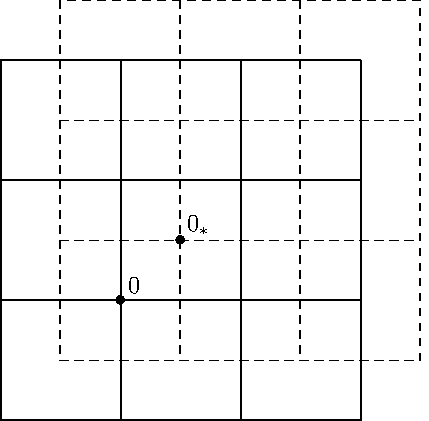
\includegraphics{du1}

\eec

\vs

Notemos que há uma relação 1 a 1 entre os sítios e elos de $\zt$ e aqueles
de $\zs$. Seja a relação (1 a 1) $e\to\es$ entre elos de $\zt$ e $\zs$ que associa 
a cada elo da primeira rede o elo secante da rede dual, como na figura a
seguir.

\bec
%\input sec.tex
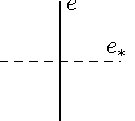
\includegraphics{sec}
\eec

Definiremos um modelo de percolação em $\zs$ induzido pelo modelo em $\zt$
declarando $\es$ aberto ou fechado conforme $e$ esteja aberto ou fechado,
respectivamente.

No que se segue, um {\em circuito} será um caminho $\{e_1,e_2,\ldots,e_n\}$
tal que $y_n=x_1$, isto é, um caminho que se fecha sobre si mesmo.

A ocorrência de um aglomerado da origem finito em $\zt$ está associada à
existência de um circuito fechado (isto é, um circuito de elos fechados) na
rede dual ao redor da origem. Isto se deve ao fato de que se o aglomerado da
origem for finito, os elos da fronteira do aglomerado (isto é, elos ligando
sítios do aglomerado a sítios fora do aglomerado), obviamente fechados, estão
sempre dispostos de tal forma que os elos correspondentes do dual formam um 
circuito, que será então fechado. A figura a seguir ilustra este fato geométrico
elementar, bastante
intuitivo (o aglomerado da origem aparece em linhas cheias, sua fronteira em linhas
pontilhadas e o circuito no dual em linhas tracejadas) e, como a
prova é longa e tediosa (vide \cite{kn:K2} página 386 e
a Proposição~\ref{pro:geo} na página~\pageref{pro:geo} destas notas), 
não a apresentaremos neste texto.

\vs

\bec

%\input cir.tex
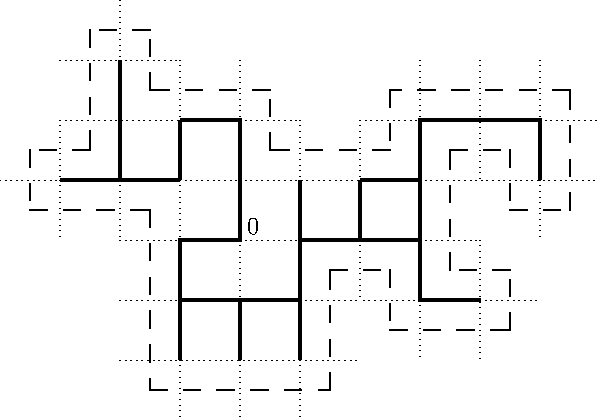
\includegraphics{cir}

\eec

\vs

Seguimos com a demonstração da Proposição \ref{prop:trans2}.

Vamos mostrar que a probabilidade de o aglomerado da origem ser finito
é estritamente menor do que 1 para $p$ suficientemente próximo de 1. Para
isto, em vista do fato geométrico acima, bastará argumentar que a probabilidade
de haver algum circuito fechado na rede dual ao redor da origem é estritamente
menor do que 1 para $p$ suficientemente próximo de 1. O argumento é semelhante
ao {\em argumento de Peierls} para demonstrar a ocorrência de magnetização no
modelo de Ising.
\beqnn
\p(\mbox{há um circuito fechado na rede dual ao redor da origem})\\
\leq\sum_{\ga}\p(\ga\,\mbox{está fechado}),
\quad\quad\quad\quad\quad\quad\quad\quad\quad
\eeqnn 
onde a soma é sobre todos os circuitos $\ga$ ao redor da origem. Ela pode ser
reordenada da seguinte maneira
$$
\sum_{n\geq4}\sum_{|\ga|=n}\p(\ga\,\mbox{está fechado}),
$$
onde a segunda soma é sobre circuitos $\ga$ ao redor da origem de comprimento $n$.

Está claro que a probabilidade no interior das somas depende apenas de $n$ e vale
$(1-p)^n$. Portanto, a expressão acima fica
$$
\sum_{n\geq4}\ln(1-p)^n,
$$
onde $\ln$ denota o número de circuitos na rede dual ao redor da origem de 
comprimento $n$.

O seguinte argumento produz uma cota superior útil para $\ln$. Qualquer circuito
de comprimento $n$ da rede dual ao redor da origem deve cruzar um elo da rede
original da forma $((0,k),(0,k+1))$, para algum $-n/2\leq k\leq n/2$. A partir deste
elo secante, cada um dos $n-1$ elos subseqüentes pode ser colocado de no máximo 
$3$ maneiras diferentes. Por isto
$$\ln\leq n3^{n-1}.$$
Substituindo na soma acima, temos
$$
\sum_{n\geq4}\frac{n}{3}[3(1-p)]^n,
$$
que é uma função contínua e decrescente em $p$ quando $p>2/3$, anulando-se 
quando $p=1$. Segue-se que existe $p_0<1$ tal que a expressão acima é
estritamente menor do que 1 para $p>p_0$.$\bo$

\vs

Uma melhoria do argumento acima que mostra que a probabilidade de o aglomerado
da origem ser infinito ($\tep$) é
estritamente positiva para $p>2/3$ é o seguinte.
   
Denotemos por $Q_M$ o quadrado centrado na origem e de lado $2M+1$.
Seja $A_M$ o evento que todos os elos de $Q_M$ estejam abertos e
$B_M$ o evento de haver um circuito fechado na rede dual {\em completamente
fora de} $Q_M$.

Repetindo o argumento da demonstração acima, temos
$$
\p(B_M)\leq\sum_{n\geq 8M+4}\frac{n}{3}[3(1-p)]^n.  
$$
Dado $p>2/3$, esta expressão pode ser tornada estritamente menor do que 1 
escolhendo-se $M$ suficientemente grande, digamos $M_0$. Portanto
\beq\label{eq:pei}\p(B_{M_0}^c)>0.\eeq

Agora, na intersecção dos eventos $A_{M_0}$ e $B_{M_0}^c$, o aglomerado da origem é
infinito. Além disso, $A_{M_0}$ e $B_{M_0}^c$ são independentes, pois dependem de
conjuntos disjuntos de elos. Logo, de (\ref{eq:pei}) concluimos que
$$
\tep\geq\p(A_{M_0}\cap B_{M_0}^c)=\p(A_{M_0})\p(B_{M_0}^c)>0,
$$
pois $\p(A_{M_0})>0$ (ainda que próximo de 0). O argumento está completo. 

\vs

A probabilidade crítica $\pce$ depende da dimensão e podemos denotá-la
$\pce(d)$. As proposições acima mostram que 
$$\frac{1}{2d-1}\leq\pce(d)\leq\frac{2}{3}.$$ Kesten~\cite{kn:K3} mostrou que
$$\pce(d)\sim\frac{1}{2d}$$ para dimensões grandes.

\vs

O Teorema~\ref{teo:trans} não diz nada sobre o que acontece em $p=\pce$.
Como veremos no Capítulo~4, $\tep$ é uma função contínua, exceto possivelmente
em $p=\pce$. Se $\tepc=0$, então $\tep$ será contínua e seu gráfico se
parecerá com o da figura à esquerda a seguir.
Caso contrário, o gráfico será mais parecido com o da figura à direita.

\vs
%\input cont
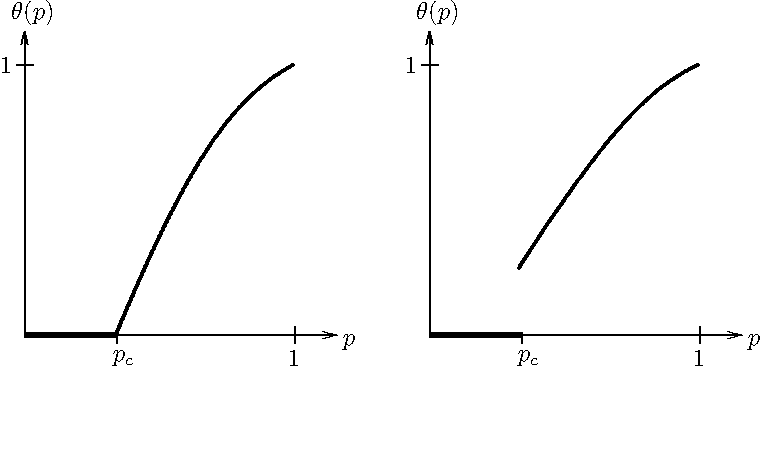
\includegraphics{cont}

Qual caso vale é uma questão em aberto para $d$ genérico, mas se acredita que $\tep$ seja
contínua. Isto está de fato provado em 2 dimensões e em dimensões grandes.
Veremos o caso bidimensional no Capítulo~5 e discutiremos um método de
ataque ao problema em mais dimensões no Capítulo~6.




\chapter{Ferramentas úteis}
\setcounter{equation}{0}
\label{chp:fer}
Este capítulo será dedicado à apresentação de alguns resultados auxiliares 
a serem utilizados nos capítulos subseqüentes.
Todos dizem respeito a funções e eventos {\em crescentes}, que passamos a definir.

Para isto, introduzimos a ordem parcial em $\Om$
$$\om\leq\om'\Leftrightarrow\ \om_e\leq\om'_e\,\,\mbox{para todo $e\in\ed$}.$$ 

Uma variável aleatória $X$
é dita crescente se for crescente na ordem parcial acima, isto é,
$$X(\om)\leq X(\om')\,\,\mbox{sempre que}\,\,\om\leq\om'.$$ 
Um evento $A\in{\cal E}$ é dito crescente se $\ind_A$, a função indicadora
de $A$, for crescente.

Em palavras, um evento $A$ é crescente sempre que para cada configuração de
elos abertos em que $A$ ocorre, ao abrirmos mais elos nesta configuração,
$A$ continua ocorrendo. Exemplos comuns são os eventos $\{x\lr y\}$ em 
que dois sítios da rede estão conectados por um caminho de elos abertos
e $\{\cl=\infty\}$ em que o aglomerado da origem é infinito. 

\section{Desigualdade de FKG}
\setcounter{equation}{0}
\label{sec:fkg}
Eventos e, mais geralmente, variáveis aleatórias crescentes do modelo de percolação
têm a propriedade de serem positivamente correlacionadas.
 
\vfill\eject

\bteo[Desigualdade de FKG]
\label{teo:fkg}
Sejam $Z$ e $Y$ duas variáveis a\-le\-a\-tó\-rias crescentes e limitadas em $\Om$.
Então
\beq
\ep(ZY)\geq\ep(Z)\ep(Y).
\eeq
\eteo

\vs

\noindent{\bf Prova do Teorema \ref{teo:fkg}}

Vamos supor inicialmente que $Z$ e $Y$ sejam cilíndricas, isto é, dependam apenas 
de um conjunto finito de
elos $\{e_1,e_2,\ldots,e_n\}$. Provaremos o teorema neste caso por indução em
$n$.

Para $n=1$, $Z=f(X_{e_1})$ e $Y=g(X_{e_1})$, onde $f$ e $g$ são crescentes.
Seja $Y'$ uma cópia independente de $X_{e_1}$ (isto é, $Y'$ e $X_{e_1}$ são
i.i.d.). Então
$$[f(X_{e_1})-f(Y')][g(X_{e_1})-g(Y')]\geq0,$$
pelo fato de $f$ e $g$ serem crescentes. Portanto
$$\ep\left\{[f(X_{e_1})-f(Y')][g(X_{e_1})-g(Y')]\right\}\geq0.$$
Expandindo o termo à esquerda, temos
\beqn\nonumber&&\ep[f(X_{e_1})g(X_{e_1})]+\ep[f(Y')g(Y')]\\ \label{eq:f1}\ge
\ep[f(X_{e_1})g(Y')]+\ep[f(Y')g(X_{e_1})].\eeqn Pela independência entre 
$X_{e_1}$ e $Y'$, a expressão à direita fica
$$\ep[f(X_{e_1})]\ep[g(Y')]+\ep[f(Y')]\ep[g(X_{e_1})].$$
Como $X_{e_1}$ e $Y'$ têm a mesma distribuição, a desigualdade (\ref{eq:f1})
fica
\beqnn&&\ep[f(X_{e_1})g(X_{e_1})]+\ep[f(X_{e_1})g(X_{e_1})]\\ \ge
\ep[f(X_{e_1})]\ep[g(X_{e_1})]+\ep[f(X_{e_1})]\ep[g(X_{e_1})],\eeqnn
isto é
$$2\ep[f(X_{e_1})g(X_{e_1})] \geq
2\ep[f(X_{e_1})]\ep[g(X_{e_1})]$$
e o resultado está provado para $n=1$. 

Supondo-o válido para $n=k$, seja $n=k+1$. Então 
$$Z=f(X_{e_1},\ldots,X_{e_k},X_{e_{k+1}})\quad\mbox{e}\quad
Y=g(X_{e_1},\ldots,X_{e_k},X_{e_{k+1}}),$$ com $f$ e $g$ crescentes.

Agora
\beqnn
\ep(ZY)\=\ep\left[f(X_{e_1},\ldots,X_{e_k},X_{e_{k+1}})
g(X_{e_1},\ldots,X_{e_k},X_{e_{k+1}})\right]\\
\=\ep\left\{\ep\left[f(X_{e_1},\ldots,X_{e_k},X_{e_{k+1}})
g(X_{e_1},\ldots,X_{e_k},X_{e_{k+1}})|X_{e_{k+1}}\right]\right\}.
\eeqnn
Na esperança condicional acima, $X_{e_{k+1}}$ está fixo e portanto
$f$ e $g$ podem ser vistas como funções de $X_{e_1},\ldots,X_{e_k}$
e a hipótese de indução pode ser aplicada para dar que a última 
expressão acima é maior ou igual a 
$$\ep\left\{\ep\left[f(X_{e_1},\ldots,X_{e_k},X_{e_{k+1}})|X_{e_{k+1}}\right]
\ep\left[g(X_{e_1},\ldots,X_{e_k},X_{e_{k+1}})|X_{e_{k+1}}\right]\right\}.$$
Agora é claro que as esperanças condicionais acima são funções crescentes
de $X_{e_{k+1}}$. Novo uso da hipótese de indução produz o resultado para
$n=k+1$, completando o passo de indução.

Para completar a demonstração, consideremos $Z$ e $Y$ não necessariamente
cilíndricas. Seja $e_1,e_2,\ldots$ uma enumeração de $\ed$. Pelo Teorema da
Convergência de Martingais (veja \cite{kn:B}),
$$Z=\lim_{n\to\infty}\ep\left[Z|X_{e_1},\ldots,X_{e_n}\right]$$
e de maneira semelhante para $Y$.
Pelo passo anterior, a desigualdade de FKG vale quando $Z$ e $Y$ são substituidos
por $$\ep\left[Z|X_{e_1},\ldots,X_{e_n}\right]\quad\mbox{e}\quad 
\ep\left[Y|X_{e_1},\ldots,X_{e_n}\right].$$ Uma passagem ao limite em $n$ e o Teorema
da Convergência Dominada nos dão o resultado geral. $\bo$

\vs

\bcor
\label{cor:fkg}
Se $A$ e $B$ forem eventos crescentes, então
\beq
\label{eq:fkg}
\p(A\cap B)\geq\p(A)\p(B).
\eeq
\ecor

\vs

\noindent{\bf Prova}

Basta aplicar o Teorema \ref{teo:fkg} com $Z=\ind_A$ e $Y=\ind_B$ $\bo$

\vs

Observamos que a desigualdade em (\ref{eq:fkg}) é equivalente a
$$\p(A|B)\geq\p(A),$$ 
o que nos diz que a ocorrência de um evento crescente aumenta a probabilidade
de ocorrência de um outro evento crescente.

\vs

O Teorema~\ref{teo:fkg} vale também para duas v.a.'s 
decrescentes (na ordem parcial), pois a desigualdade não muda se substituirmos $Z$ e $Y$ respectivamente
por $-Z$ e $-Y$, que são crescentes. Segue que o Corolário~\ref{cor:fkg} vale
também para dois eventos decrescentes.

\vs

As desigualdades acima foram primeiro provadas por Harris \cite{kn:H} e
posteriormente generalizadas para outros modelos por Fortuin, Kasteleyn e
Ginibre \cite{kn:FKG}, cujas iniciais batizaram-nas.

\section{Desigualdade de BK}
\setcounter{equation}{0}
\label{sec:bk}
A próxima desigualdade que discutiremos vai no sentido contrário da
desigualdade de
FKG e envolve uma intersecção {\em restrita} de eventos crescentes.

Dados dois eventos crescentes $A$ e $B$ de ${\cal E}$, dizemos que $A$ e $B$ ocorrem 
{\em disjuntamente} (para um dado $\om$) se existirem dois caminhos abertos (de elos)
disjuntos (em $\om$) tais que o primeiro garante a ocorrência de $A$ e o segundo 
garante a ocorrência de $B$.
Denotamos por $A\circ B$ a ocorrência disjunta de $A$ e $B$.

Por exemplo, no evento $\{x\lr y\}\circ\{u\lr v\}$ há dois caminhos abertos disjuntos,
um ligando os sítios $x$ e $y$ e outro ligando os sítios $u$ e $v$.

\vs

\bteo[Desigualdade de BK]

Sejam $A$ e $B$ dois eventos crescentes de ${\cal E}$
dependendo apenas de um conjunto finito de elos. Então
$$
\p(A\circ B)\leq\p(A)\p(B).
$$
\eteo

\vs

O nome da desigualdade é referência a seus descobridores van den Berg e 
Kesten \cite{kn:vBK}.
A restrição a eventos que dependem apenas de um conjunto finito de elos
deve-se a
razões técnicas, a extensão pode ser feita para outros casos de interesse.
Para uma discussão mais completa com a demonstração do resultado, veja
\cite{kn:G} página 29. Discutiremos abaixo a idéia da prova, usando os eventos
do exemplo acima, mas restritos a uma sub-rede finita de $\zd$ (por exemplo, o quadrado 
$Q_M$ do capítulo anterior, para algum $M$), do contrário eles dependerão de um 
conjunto infinito de elos.

Notemos para começar que dada a ocorrência de $\{u\lr v\}$, temos informação
sobre elos abertos, que {\em não podem} ser usados na ocorrência disjunta de
$\{x\lr y\}$. Isto torna plausível a desigualdade
$$\p(\{x\lr y\}\circ\{u\lr v\}|u\lr v)\leq\p(x\lr y).$$

A idéia da prova é a seguinte. Seja ${\cal G}$ uma sub-rede finita de $\zd$ e $e$ um
elo de ${\cal G}$. Substituamos $e$ por dois elos paralelos 
$e'$ e $e''$ abertos com probabilidade $p$ e fechados com probabilidade $1-p$
independentemente um do outro. Considera-se a ocorrência disjunta de 
$\{x\lr y\}$ e $\{u\lr v\}$ nesta nova rede, mas com o primeiro evento evitando
$e''$ e o segundo evento evitando $e'$. Observa-se que esta operação não pode
diminuir a probabilidade original. Continua-se
indutivamente substitindo-se os elos $f$ de ${\cal G}$ por elos paralelos 
e independentes
$f'$ e $f''$ e considerando-se a ocorrência disjunta de $\{x\lr y\}$ e $\{u\lr v\}$
na nova rede, a ocorrência do primeiro sem usar elos $''$ e a do segundo
sem usar elos $'$. A operação não diminui a probabilidade do passo anterior. 
Ao término, esgotados todos os elos de ${\cal G}$, temos
duas cópias independentes desta rede, uma na qual perguntamos pela ocorrência de
$\{x\lr y\}$, na outra perguntamos pela ocorrência de
$\{u\lr v\}$, eventos portanto independentes. A probabilidade final é então o produto
das probabilidades dos eventos e a cadeia de desigualdades levando à probabilidade
de ocorrência disjunta dos eventos em ${\cal G}$ nos dá o resultado.

\begin{defin}
\label{def:con}
À probabilidade de que dois sítios $x$ e $y$ estejam conectados por um caminho
aberto, $$\p(x\lr y),$$
chamamos {\em função de conectividade} (entre $x$ e $y$), com a notação
$\tp(x,y).$
\end{defin}

\section{Fórmula de Russo}
\setcounter{equation}{0}
\label{sec:rus}
O próximo resultado é uma fórmula para a derivada em $p$ da probabilidade de
um evento crescente. Para obtê-la, usaremos a construção acoplada do modelo
de percolação
usando a família de variáveis uniformes ${\cal Z}$ vista no capítulo anterior
(o modelo padrão).

Consideramos então, para uma dada configuração das variáveis em ${\cal Z}$, a
configuração de elos $p$-abertos $\op$, isto é, $(\op(e))_{e\in\ed}$ tal que 
$$\op(e)=\cases{1,& se $Z_e<p$\cr
                0,& caso contrário}$$
para todo $e\in\ed$.

Seja $A$ um evento crescente que depende de um conjunto finito de elos $\g$ de
$\ed$ e considere
\beq
\label{eq:r1}
\ppd(A)-\p(A)=\pp(\op\notin A, \opd\in A).
\eeq

Se $A$ é crescente, $\op\notin A$ e $\opd\in A$, então há elos $e$ tais que
$\op(e)=0$ mas $\opd(e)=1$, isto é, $p\leq Z_e<p+\d$. Denote por $\epd$ o
conjunto de tais elos. A probabilidade de que $|\epd|\geq2$ é $o(\d)$.
Por outro lado, se $\op\notin A$, $\opd\in A$ e $|\epd|=1$, então o (estado do) elo $e$ em questão deve ser {\em
essencial} em $\op$ 
para (a ocorrência ou não de) $A$ no sentido de que $\op\notin A$, mas $\op'\in A$, onde $\op'$ é a
configuração obtida de $\op$ trocando o status do elo $e$ de $0$ para $1$. 
A última probabilidade em (\ref{eq:r1}) fica, então,
$$\pp(\op\notin A, \opd\in A,|\epd|=1)+o(\d).$$

A probabilidade acima pode ser escrita como
$$
\sum_{e\in\g}\pp(\op\notin A, \opd\in A,\epd=\{e\}).
$$

O evento dentro da probabilidade na soma é equivalente ao evento
$$
\{\mbox{$e$ é essencial em $\op$ para $A$},p\leq Z_e<p+\d,\epd=\{e\}\}.
$$
Aquela probabilidade pode ser escrita, então, como
\beqn
\label{eq:piv1}
\mbox{}\!\!\!\!\!\!\!\!&&\pp[\mbox{$e$ é essencial em $\op$ para $A$},p\leq
Z_e<p+\d]\\
\label{eq:piv2}
\mbox{}\!\!\!\!\!\!\!\!&-&\pp[\mbox{$e$ é essencial em $\op$ para $A$},p\leq
Z_e<p+\d,\epd\ne\{e\}].
\eeqn

A probabilidade em~(\ref{eq:piv2}) é limitada superiormente por
$$\pp(|\epd|\geq2)=o(\d).$$

Observemos agora que o evento \{$e$ é essencial em $\op$ para $A$\} não depende de $e$.
Logo, a probabilidade em~(\ref{eq:piv1}) fatora. 

Combinando os argumentos acima, temos
\beqnn
\ppd(A)-\p(A)\=\sum_e\pp(\mbox{$e$ é essencial em $\op$ para $A$})\pp(p\leq Z_e<p+\d)+o(\d)\\
             \=\d\sum_e\pp(\mbox{$e$ é essencial em $\op$ para $A$})+o(\d)\\
             \=\d E(N(A))+o(\d),
\eeqnn
onde $N(A)$ denota o número de elos essenciais em $\op$ para $A$ (e
$E$ é a esperança com respeito a $\pp$).

Modificando um pouco a terminologia, e voltando ao modelo com as variáveis de
Bernoulli, dado um evento qualquer $A\in\e$ e uma configuração $\om\in\Om$, 
definimos um elo $e$ como {\em pivotal} para $A$ (mais precisamente, para
($A,\om$)) se, denotando por
$\om'$ a configuração idêntica a $\om$ em todos os elos com exceção de $e$, em
que $\om$ e $\om'$ são diferentes, uma das duas coisas acontece: ou
$$\om\in A\quad\mbox{e}\quad\om'\notin A$$
ou
$$\om\notin A\quad\mbox{e}\quad\om'\in A.$$

Seja $N(A)$ o número de elos pivotais para $A$. O argumento acima prova o seguinte.

\vs

\bteo {\bf Fórmula de Russo~\cite{kn:R}}

Se $A$ for um evento crescente dependendo de um conjunto finito de elos,
então
\beq
\label{eq:rus}
\frac{d}{dp}\p(A)=\ep(N(A)).
\eeq
\eteo  

\vs

A equação (\ref{eq:rus}) também pode ser escrita
$$
\frac{d}{dp}\p(A)=\sum_{e}\p(\mbox{$e$ é pivotal para $A$}).
$$

O uso que se fará da fórmula de Russo parte da observação de
que o evento \{$e$ é pivotal para $A$\} é independente do elo $e$ e portanto
independente do evento \{$e$ está aberto\}, para deduzir que
$$
\p(\mbox{$e$ é pivotal para $A$})=
\frac{1}{p}\p(\mbox{$e$ está aberto e é pivotal para $A$}).
$$

Logo, se $A$ for crescente, aplicando a fórmula de Russo temos
\beqn
\frac{d}{dp}\p(A)\=\frac{1}{p}\sum_{e}\p(\mbox{$e$ está aberto e é pivotal para $A$})\\
\=\frac{1}{p}\sum_{e}\p(A\cap\{\mbox{$e$ é pivotal para $A$}\})\\
\=\frac{1}{p}\sum_{e}\p(A)\p(\mbox{$e$ é pivotal para $A$}|A)\\
\=\frac{1}{p}\ep(N(A)|A)\p(A).
\eeqn

Dividindo a primeira e última expressões por $\p(A)$ e integrando em
$[p_1,p_2]$ ($0< p_1\leq p_2\leq1$), chegamos a
\beq
P_{p_2}(A)=P_{p_1}(A)\exp\left(\int_{p_1}^{p_2}\frac{1}{p}\ep(N(A)|A)dp\right).
\eeq

A identidade acima será aplicada no próximo capítulo.

\chapter{Fase Subcrítica: Decaimento Exponencial}
\renewcommand{\theequation}{\thechapter .\arabic{equation}}
\pagestyle{myheadings}
\markboth{CAPÍTULO 3.\quad FASE SUBCRÍTICA}{DECAIMENTO EXPONENCIAL}
\setcounter{equation}{0}
\label{chp:exp}
Poderíamos definir outros pontos críticos no modelo de percolação. Por exemplo,  
lembrando que $\xip$ é o valor esperado do volume do aglomerado aberto da origem, 
seja 
\beq 
\pt=\sup\{p:\xip<\infty\}. 
\eeq 
A prova da Proposição~\ref{prop:trans1} mostra que $\pt$ está bem definido e é
positivo.
É claro que $\pt\leq p_c$ (pois se $\tep=\p(|C|=\infty)>0)$ então $\xip=\infty$). 
 
Neste capítulo,  veremos que $\pt=\pce$, eliminando a existência de uma fase 
intermediária $(\pt,\pce)$ e estabelecendo a assim chamada {\em unicidade} do ponto 
crítico. 
 
Este resultado foi provado independentemente por Menshikov \cite{kn:M} e  
Aizenman e Barsky \cite{kn:AB} por argumentos diferentes (para $d$ geral; em 2 dimensões foi provado 
por Kesten \cite{kn:K1} como conseqüência de que, neste caso, $\pce=1/2$). Mostraremos a seguir o 
argumento de Menshikov (com uma melhoria de Kesten, não publicada). 
 
Sejam $\sn$ a esfera $L_1$  em $\zd$ de raio $n$ com centro na origem, isto é 
$$\sn=\{x\in\zd:||x||_1\leq n\}$$ e  $A_n$ o evento de que existe um caminho 
aberto da origem à fronteira de $\sn$. 

\vs

\bte[Menshikov]
\label{teo:teo1} 
Se $p<\pce$, então para algum $\psp>0$ 
\beq 
\label{eq:exp0}
\p(A_n)\leq e^{-\psp n}\quad\mbox{para todo $n$.} 
\eeq  
\ete 

%\nopagebreak
 
\vs

\bco
\label{cor:exp}
$\xip<\infty$ se $p<\pce$.
\eco

\vs

\bob
Na fase supercrítica $\xip=\infty$, obviamente.
Prova-se tam\-bém \cite{kn:G} que $$\lim_{p\ua\pce}\xip=\infty.$$
\eob

\vs

\noindent {\bf Prova do Corolário~\ref{cor:exp}.}

O Teorema~\ref{teo:teo1} estabelece o decaimento exponencial da distribuição
do raio de $C$.
De~(\ref{eq:exp0}) concluimos que 
\beq
\label{eq:exp1}
\p(|C|\geq n)\leq e^{-\psp' n^{1/d}},
\eeq
com $\psp'>0$. Logo,
$$\xip=\sum_{n\geq1}\p(|C|\geq n)<\infty. \bo$$

\vs

\bob
\label{ob:exp1}
(\ref{eq:exp1}) estabelece decaimento subexponencial da distribuição de 
$|C|$. Com um pouco mais de trabalho, mostra-se o decaimento exponencial desta
distribuição (vide~\cite{kn:G}).
\eob

\vs

A prova do Teorema~\ref{teo:teo1} será  apresentada em uma introdução mais 
três partes. 
 
\vspace{.5cm} 
 
\noindent {\bf Introdução} 
 
Defina 
\beq 
\gpn=\p(A_n). 
\eeq 
 
Note que $\gpn\da\tep$ quando $n\ua\infty$. Logo, se $p<\pce$, existe $p'$ satisfazendo 
$p<p'<\pce$ e portanto $$\lim_{n\to\infty}g_{p'}(n)=\theta(p')=0.$$ 
O problema é mostrar que para algum $p'$, se  
$\lim_{n\to\infty}g_{p'}(n)=0$ então para $p<p'$ 
$$\gpn\leq e^{-\psp n}.$$ 
Queremos limitar $\gpn$ superiormente em termos de $g_{p'}(n)$ e mais alguma coisa 
(é preciso melhorar a cota trivial $\gpn\leq g_{p'}(n)$). 
 
\vspace{.5cm} 
 
\noindent {\bf Parte 1} 
 
Como já vimos no Capítulo 2, Seção 3, a fórmula de Russo produz a  
seguinte desigualdade para $0<\a\leq\b\leq1$. 
\beq 
\gan\leq\gbn\exp\left(-\int_{\a}^{\b}\ep(N(A_n)|A_n)dp\right), 
\eeq 
onde $N(A_n)$ é o número de elos pivotais para o evento $A_n$. 
 
\vspace{.5cm} 
 
\noindent {\bf Parte 2} 
 
Para um dado $\b$, seja $M$ o raio (aleatório) do aglomerado aberto da 
origem (isto é, $\max_{x\in C}||x||_1$ ou, equivalentemente,  
$\max\{k:A_k$ ocorre\}). Note que se $\tep>0$, então $M=\infty$ com 
probabilidade positiva e se $\tep=0$ então $M$ é uma variável aleatória 
finita com valores inteiros.  
 
Sejam $M_1,M_2,\ldots$ variáveis aleatórias independentes 
com a mesma distribuição de $M$. Mostraremos mais adiante  
que  
\beq 
\p(N(A_n)\geq k|A_n)\geq P((1+M_1)+\ldots+(1+M_k)\leq n), 
\eeq 
para todo $k\geq0$, o que relaciona $N(A_n)$ (condicionado a  
$A_n$) a um processo de 
renovação. Usando métodos usuais em tais processos, conclui-se que 
\beqn
\nonumber
\ep(N(A_n)|A_n)\=\sum_{k=1}^\infty\p(N(A_n)\geq k|A_n)\\ 
\nonumber
\ge \sum_{k=1}^\infty P((1+M_1)+\ldots+(1+M_k)\leq n)\\ 
\label{eq:wald}
\ge \frac{n}{E(1+M\wedge n)}-1=\frac{n}{\sum_{i=0}^n\gpi}-1. 
\eeqn 

 
\vspace{.5cm} 
 
\noindent {\bf Parte 3} 
 
Combinam-se as partes 1 e 2 para obter para $0<\a\leq\b\leq1$: 
 
\beq 
\label{eq:eq3} 
\gan\leq\gbn\exp\left[(\b-\a)-(\b-\a)\frac{n}{\sum_{i=0}^n g_\beta(i)}\right]. 
\eeq 
 
Da desigualdade acima, concluiremos que  
\beq 
\label{eq:eq4} 
\sum_{i=0}^\infty g_\beta(i)<\infty, 
\eeq 
do que segue o teorema. 
 
\vspace{.5cm} 
 
Em seguida apresentaremos as partes 2 e 3 em detalhes. 
 
\vspace{.5cm} 
 
\noindent {\bf Parte 2} 
 
Sejam $\{e_1,e_2,\ldots,e_m\}$ os elos pivotais abertos para $A_n$ na ordem 
com que são atingidos por um caminho aberto da origem  
até $\del S_n$. (Note que a ordem é a mesma para qualquer tal caminho devido 
à pivotalidade.) Escreva $e_j$ como $(x_j,y_j)$ (Na "ordem correta". 
Veja a Figura~\ref{fig:exp1}.). 

\bef
%\font\thinlinefont=cmr5
\mbox{\beginpicture
\setcoordinatesystem units < 0.800cm, 0.800cm>
\unitlength= 0.800cm
\linethickness=1pt
\setplotsymbol ({\makebox(0,0)[l]{\tencirc\symbol{'160}}})
\setshadesymbol ({\thinlinefont .})
\setlinear
%
% Fig POLYLINE object
%
\linethickness= 0.500pt
\setplotsymbol ({\thinlinefont .})
\plot  3.778 16.542  3.778 16.542 /
%
% Fig POLYLINE object
%
\linethickness= 0.500pt
\setplotsymbol ({\thinlinefont .})
\putrule from  3.778 16.542 to  3.778 16.542
%
% Fig POLYLINE object
%
\linethickness=1pt
\setplotsymbol ({\makebox(0,0)[l]{\tencirc\symbol{'160}}})
\plot  7.588 16.542 12.033 20.987 /
%
% Fig POLYLINE object
%
\linethickness=1pt
\setplotsymbol ({\makebox(0,0)[l]{\tencirc\symbol{'160}}})
\plot 12.033 20.987 16.478 16.542 /
%
% Fig POLYLINE object
%
\linethickness= 0.500pt
\setplotsymbol ({\thinlinefont .})
%
% arrow head
%
\plot 12.097 21.368 12.033 21.622 11.970 21.368 /
%
\putrule from 12.033 21.622 to 12.033 11.462
%
% Fig POLYLINE object
%
\linethickness=1pt
\setplotsymbol ({\makebox(0,0)[l]{\tencirc\symbol{'160}}})
\plot  7.588 16.542 12.033 12.097 /
%
% Fig POLYLINE object
%
\linethickness=1pt
\setplotsymbol ({\makebox(0,0)[l]{\tencirc\symbol{'160}}})
\plot 16.478 16.542 12.033 12.097 /
%
% Fig POLYLINE object
%
\linethickness=1pt
\setplotsymbol ({\makebox(0,0)[l]{\tencirc\symbol{'160}}})
\putrule from 12.668 18.447 to 10.741 18.447
\putrule from 10.763 18.447 to 10.763 17.790
\putrule from 10.763 17.812 to 12.668 17.812
%
% Fig POLYLINE object
%
\linethickness=1pt
\setplotsymbol ({\makebox(0,0)[l]{\tencirc\symbol{'160}}})
\putrule from 10.763 17.812 to 10.763 15.272
%
% Fig POLYLINE object
%
\linethickness=1pt
\setplotsymbol ({\makebox(0,0)[l]{\tencirc\symbol{'160}}})
\putrule from 10.763 16.542 to  9.471 16.542
\putrule from  9.493 16.542 to  9.493 15.250
\putrule from  9.493 15.272 to 14.573 15.272
%
% Fig POLYLINE object
%
\linethickness=1pt
\setplotsymbol ({\makebox(0,0)[l]{\tencirc\symbol{'160}}})
\putrule from 11.398 15.272 to 11.398 12.732
%
% Fig POLYLINE object
%
\linethickness=0pt
\setplotsymbol ({\thinlinefont \ })
\putrule from 13.303  9.557 to 14.573  9.557
%
% Fig POLYLINE object
%
\linethickness=0pt
\setplotsymbol ({\thinlinefont \ })
\putrule from 13.303  9.557 to 14.573  9.557
%
% Fig POLYLINE object
%
\linethickness=0pt
\setplotsymbol ({\thinlinefont \ })
\putrule from 19.018 15.907 to 19.018 11.462
%
% Fig POLYLINE object
%
\linethickness=0pt
\setplotsymbol ({\thinlinefont \ })
\putrule from  8.223  9.557 to 10.763  9.557
%
% Fig POLYLINE object
%
\linethickness=1pt
\setplotsymbol ({\makebox(0,0)[l]{\tencirc\symbol{'160}}})
\putrule from 12.668 18.447 to 12.668 16.542
%
% Fig POLYLINE object
%
\linethickness=1pt
\setplotsymbol ({\makebox(0,0)[l]{\tencirc\symbol{'160}}})
\putrule from 12.668 17.177 to 12.011 17.177
\putrule from 12.033 17.177 to 12.033 16.520
\putrule from 12.033 16.542 to 12.668 16.542
%
% Fig POLYLINE object
%
\linethickness=1pt
\setplotsymbol ({\makebox(0,0)[l]{\tencirc\symbol{'160}}})
\putrule from 14.573 15.272 to 14.573 14.637
%
% Fig POLYLINE object
%
\linethickness=1pt
\setplotsymbol ({\makebox(0,0)[l]{\tencirc\symbol{'160}}})
\plot 10.763 17.177 10.763 17.177 /
%
% Fig POLYLINE object
%
\linethickness= 0.500pt
\setplotsymbol ({\thinlinefont .})
\plot 10.763 17.177 10.763 17.177 /
%
% Fig POLYLINE object
%
\linethickness= 0.500pt
\setplotsymbol ({\thinlinefont .})
\putrule from  6.953 16.542 to  9.493 16.542
%
% Fig POLYLINE object
%
\linethickness= 0.500pt
\setplotsymbol ({\thinlinefont .})
\putrule from 11.398 16.542 to 17.113 16.542
%
% arrow head
%
\plot 16.859 16.478 17.113 16.542 16.859 16.605 /
%
%
% Fig POLYLINE object
%
\linethickness= 0.500pt
\setplotsymbol ({\thinlinefont .})
\setdashes < 0.1270cm>
\plot 10.763 17.177 10.922 17.177 /
%
% Fig POLYLINE object
%
\linethickness= 0.500pt
\setplotsymbol ({\thinlinefont .})
\setsolid
\putrule from 10.763 16.542 to 11.557 16.542
%
% Fig POLYLINE object
%
\linethickness=1pt
\setplotsymbol ({\makebox(0,0)[l]{\tencirc\symbol{'160}}})
\putrule from 14.573 15.907 to 14.573 15.272
%
% Fig POLYLINE object
%
\linethickness=1pt
\setplotsymbol ({\makebox(0,0)[l]{\tencirc\symbol{'160}}})
\putrule from 13.938 15.907 to 13.938 13.980
\putrule from 13.938 14.002 to 12.668 14.002
%
% Fig POLYLINE object
%
\linethickness=1pt
\setplotsymbol ({\makebox(0,0)[l]{\tencirc\symbol{'160}}})
\putrule from 12.668 12.732 to 12.668 14.659
\putrule from 12.668 14.637 to 10.741 14.637
\putrule from 10.763 14.637 to 10.763 13.980
\putrule from 10.763 14.002 to 12.033 14.002
%
% Fig POLYLINE object
%
\linethickness=1pt
\setplotsymbol ({\makebox(0,0)[l]{\tencirc\symbol{'160}}})
\putrule from 10.128 17.177 to 10.128 15.885
\putrule from 10.128 15.907 to  8.858 15.907
%
% Fig POLYLINE object
%
\linethickness=1pt
\setplotsymbol ({\makebox(0,0)[l]{\tencirc\symbol{'160}}})
\putrule from 11.398 19.082 to 11.398 17.812
%
% Fig POLYLINE object
%
\linethickness=1pt
\setplotsymbol ({\makebox(0,0)[l]{\tencirc\symbol{'160}}})
\putrule from 12.668 19.082 to 12.668 18.447
%
% Fig POLYLINE object
%
\linethickness=1pt
\setplotsymbol ({\makebox(0,0)[l]{\tencirc\symbol{'160}}})
\putrule from 12.668 16.542 to 12.668 15.907
%
% Fig POLYLINE object
%
\linethickness=1pt
\setplotsymbol ({\makebox(0,0)[l]{\tencirc\symbol{'160}}})
\putrule from 12.668 16.542 to 13.303 16.542
%
% Fig POLYLINE object
%
\linethickness=1pt
\setplotsymbol ({\makebox(0,0)[l]{\tencirc\symbol{'160}}})
\putrule from 12.668 17.177 to 13.144 17.177
%
% Fig POLYLINE object
%
\linethickness=1pt
\setplotsymbol ({\makebox(0,0)[l]{\tencirc\symbol{'160}}})
\putrule from 13.144 17.177 to 13.303 17.177
%
% Fig TEXT object
%
\put {$0$} [lB] at 11.716 16.066
%
% Fig TEXT object
%
\put {$e_1$} [lB] at 12.827 17.335
%
% Fig TEXT object
%
\put {$e_2$} [lB] at 10.922 17.335
%
% Fig TEXT object
%
\put {$e_3$} [lB] at 10.922 16.701
%
% Fig TEXT object
%
\put {$e_4$} [lB] at 10.922 15.431
\linethickness=0pt
\putrectangle corners at  3.778 21.622 and 19.018  9.557
\endpicture}

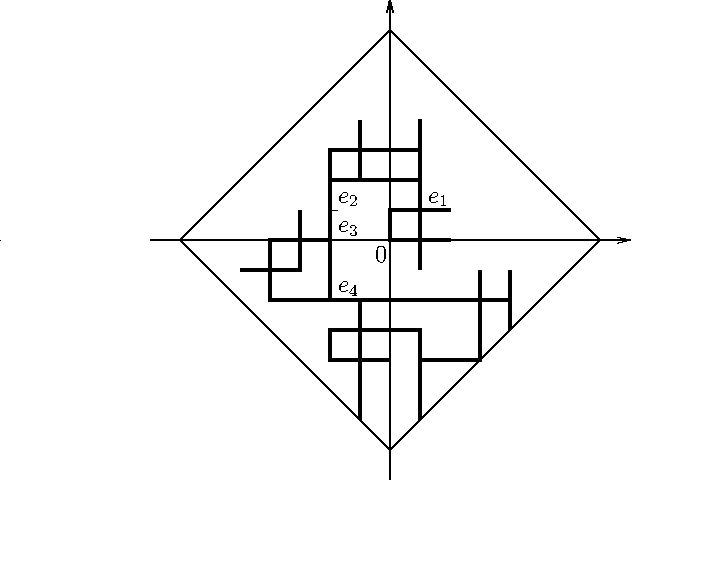
\includegraphics{piv1}
\caption{Figura do aglomerado da origem em $S_7$. Há exatamente 4 elos
pivotais para $A_7$ nesta configuração, denotados $e_1$, $e_2$, $e_3$ e $e_4$.}
\label{fig:exp1}
\eef

Os elos do aglomerado da origem entre os elos pivotais sucessivos formam
{\em salsichas}. O aglomerado da origem em $\sn$ pode ser visto então como
como salsichas de elos conectadas por elos pivotais.
 
Sejam  
\beqnn 
\ro_1\=||x_1||_1\\ 
\ro_2\=||y_1-x_2||_1\\ 
&\vdots&\\ 
\ro_m\=||y_{m-1}-x_m||_1,  
\eeqnn          
e $\rho_i=\infty$ para $i>m$.
$\rho_1,\ldots,\rho_m$ representam os {\em raios} das salsichas sucessivas.

Então $N(A_n)\geq k$ se  
$$(\ro_1+1)+(\ro_2+1)+\ldots+(\ro_k+1)\leq n,$$ ou seja, 
$$\ro_1+\ldots+\ro_k\leq n-k.$$ 
Logo, 
\beq 
\label{eq:conf}
\p(N(A_n)\geq k|A_n)\geq\p(\ro_1+\ldots+\ro_k\leq n-k|A_n). 
\eeq 

Queremos mostrar que 
\beq 
\label{eq:eq2} 
\p(\ro_1+\ldots+\ro_k\leq n-k|A_n)\geq\p(M_1+\ldots+M_k\leq n-k), 
\eeq para todo $n$ e $k$, 
onde $M_1,M_2,\ldots$ são variáveis aleatórias independentes com distribuição 
comum igual àquela do raio do aglomerado da origem (vamos denotar esta última 
v.a. por $M$). 
 
Para obter a última desigualdade, seria bom se bastasse provar 
desigualdades envolvendo probabilidades condicionais do tipo 
\beq 
\label{eq:eq1} 
\p(\ro_k\leq r_k|\ro_1=r_1,\ldots,\ro_{k-1}=r_{k-1},A_n)\geq P(M_k\leq r_k), 
\eeq para todo $n$, $k$ e $r_1+\ldots+r_k\leq n-k$. 
 
O próximo lema mostra que este é o caso. 
 
\vs

\ble 
\label{le:le1} 
A desigualdade (\ref{eq:eq1}) implica a desigualdade (\ref{eq:eq2}) 
\ele 

\vs
 
Portanto é suficiente provar o seguinte. 
 
\vs

\ble 
\label{le:le2} 
A desigualdade (\ref{eq:eq1}) é válida. 
\ele 
 
\vs

Antes de provarmos os lemas acima, vejamos porque~(\ref{eq:eq2}) implica 
no resultado da parte 2. 
 
De (\ref{eq:conf}) e (\ref{eq:eq2}), temos 
\beq 
\p(N(A_n)\geq k|A_n)\geq P((1+M_1)+\ldots+(1+M_k)\leq n). 
\eeq 
 
Consideremos $M_1',M_2',\ldots$ v.a.'s independentes com a mesma distribuição de 
$M'=1+M\wedge n$. Temos 
$$ 
\p(N(A_n)\geq k|A_n)\geq P(M_1'+\ldots+M_k'\leq n). 
$$ 
 
Agora usamos um pouco da teoria da renovação elementar. Considere um processo de 
renovação com "tempos de vida" $M_1',M_2',\ldots$ (e portanto instantes de renovação 
$M_1'$, $M_1'+M_2',\ldots,M_1'+\ldots +M_k',\ldots$) 
 
Defina a v.a. $K$ como  1 mais o número de renovações até o instante $n$, isto é, 
$$K=\min\{k:M_1'+\ldots+M_k'>n\}.$$ 
Temos então 
$$P(M_1'+\ldots+M_k'\leq n)=P(K\geq k+1)=P(K-1\geq k).$$ 
 
Somando sobre $k\geq1$: 
$$\ep(N(A_n)|A_n)\geq E(K-1)=E(K)-1.$$ 
 
Para obter uma cota inferior para $E(K)$ usamos a 
{\em Identidade de Wald}~\cite{kn:B}, que diz que 
$$E(M_1'+\ldots+M_K')=E(K)E(M').$$ 
Como, claramente, $M_1'+\ldots+M_K'\geq n+1>n,$ temos imediatamente que 
$$E(K)-1>\frac{n}{E(M')}-1,$$ 
como queríamos. 
 
Vamos agora às demonstrações dos lemas. 
 
\vs

\noindent{\bf Prova do Lema~\ref{le:le1}} 
\beqnn 
&&\p(\ro_1+\ldots+\ro_k\leq n-k|A_n)\\ 
%
\=\!\!\!\!\!\!\sum_{r_1,\ldots,r_{k-1}} \!\!\!\!\!\!\p(\ro_k\leq
n-k-\sum_{i=1}^{k-1}r_i|\ro_1=r_1,\ldots,\ro_{k-1}=r_{k-1},A_n)\\
%
&&\mbox{}\hspace{1.5cm}\times\p(\ro_1=r_1,\ldots,\ro_{k-1}=r_{k-1}|A_n)\\ 
%
\ge\!\!\!\!\!\!\sum_{r_1,\ldots,k-1}
\!\!\!\!\!\!\p(M_k\leq n-k-\sum_{i=1}^{k-1}r_i) 
\p(\ro_1=r_1,\ldots,\ro_{k-1}=r_{k-1}|A_n)\\ 
%
\=\p(\ro_1+\ldots+\ro_{k-1}+M_k\leq n-k|A_n)\\
%
\=\!\!\!\!\!\!\sum_{r_1,\ldots,r_{k-2},r_k}
\!\!\!\!\!\!\p(\ro_{k-1}\leq n-k-\!\!\!\!\!\!\sum_{i=1,i\ne
k-1}^k\!\!\!\!\!\!r_i|\ro_1=r_1,\ldots,\ro_{k-2}=r_{k-2},\\ 
%
&&\mbox{}\hspace{2cm}M_k=r_k,A_n) 
\p(\ro_1=r_1,\ldots,\ro_{k-2}=r_{k-2},M_k=r_k|A_n)\\
%
\ge\!\!\!\!\!\!\sum_{r_1,\ldots,r_{k-2},r_k}\!\!\!\!\!\!\p(M_{k-1}\leq n-k-\!\!\!\!\!\!
\sum_{i=1,i\ne k-1}^k\!\!\!\!\!\!r_i)\\ 
%
&&\mbox{}\hspace{1.5cm}\times\p(\ro_1=r_1,\ldots,\ro_{k-2}=r_{k-2},M_k=r_k|A_n)\\
% 
\=\p(\ro_1+\ldots+\ro_{k-2}+M_{k-1}+M_k\leq n-k|A_n)\\
% 
&\vdots&\\ 
%
\ge \p(M_1+\ldots+M_k\leq n-k),  
\eeqnn
as desigualdades acima todas seguindo de~(\ref{eq:eq1}). 
\vspace{.5cm} 
 
\noindent{\bf Prova do Lema~\ref{le:le2}} 
 
Queremos provar que   
\beq  
\p(\ro_k\leq r_k|\ro_1=r_1,\ldots,\ro_{k-1}=r_{k-1},A_n)\geq\p(M\leq r_k)  
\eeq  
quando $r_1+\ldots+r_k\leq n-k.$ Isto é equivalente a (denotando o evento  
$\{\ro_1=r_1,\ldots,\ro_{k-1}=r_{k-1}\}$ por $B$)  
\beq  
\label{eq:k}  
\p(\ro_k>r_k,B,A_n)\leq\p(M>r_k)\p(B,A_n).  
\eeq  
Note que $\{M>r_k\}=A_{r_k+1}$.  
Para $k=1$ a desigualdade se torna  
\beq  
\label{eq:um}  
\p(\ro_1>r_1,A_n)\leq\p(A_{r_1+1})\p(A_n)  
\eeq   
para $r_1\leq n-1$.  
  
No evento em que $\{\ro_1>r_1\}$, a origem está conectada por dois caminhos  
disjuntos a $x_1$ e $x_1$ está a distância pelo menos $r_1+1$ da origem  
(veja a Figura~\ref{fig:exp2}).

\bef
%\input piv2
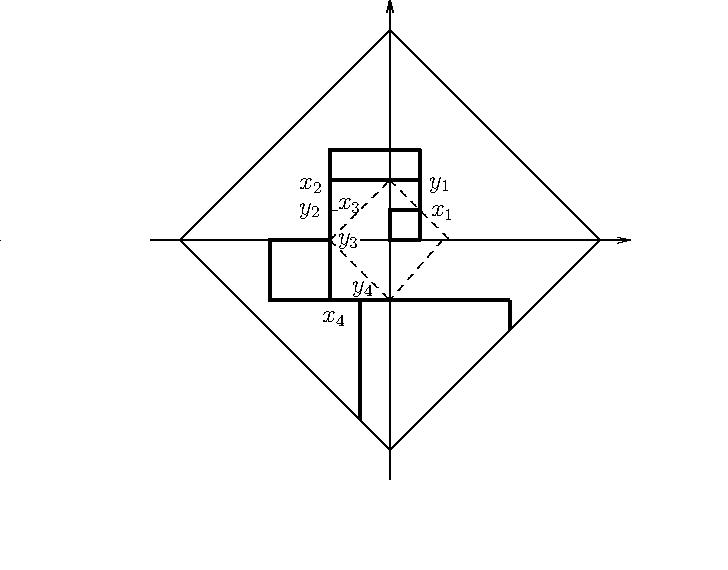
\includegraphics{piv2}
\caption{Os elos pivotais são $e_i=(x_i,y_i)$ para $i=1,2,3,4.$ Note que
$x_3=y_2$ nesta configuração. A linha tracejada é a superfície 
$\del S_{\rho_1}$ de $S_{\rho_1}$. Note os caminhos disjuntos da origem a
$\del S_{\rho_1}$.}
\label{fig:exp2}
\eef
   
No evento $\{\ro_1>r_1\}\cap A_n$, há dois caminhos disjuntos, um de $O$ a  
$\del S_{r_1+1}$ e outro de $O$ a $\del S_n$. Portanto,  
$$\{\ro_1>r_1\}\cap A_n\subset A_{r_1+1}\circ A_n$$  
e a desigualdade de BK produz a desigualdade~(\ref{eq:um}).  
  
Para $k>1$, escreva $$B=\bigcup_{\Ga}\bg,$$  
união disjunta sobre configurações (detalhadas) das salsichas até $y_{k-1}$.  
Então   
\beq  
\p(B,A_n)=\sum_\Ga\p(A_n|\bg)\p(\bg)  
\eeq  
e  
\beq  
\p(\ro_k>r_k,B,A_n)=\sum_\Ga\p(\ro_k>r_k,A_n|\bg)\p(\bg).  
\eeq  
Logo é suficiente mostrar para cada $\Ga$:  
\beq  
\p(\ro_k>r_k,A_n|\bg)\leq\p(A_{r_k+1})\p(A_n|\bg).  
\eeq  
Mas a probabilidade à esquerda é menor ou igual a  
\beqnn 
&\p(\mbox{há caminhos disjuntos abertos de $y_{k-1}$ a 
$\del S(y_{k-1},r_k+1)$ e de $y_{k-1}$}\\ 
&\mbox{}\mbox{a $\del S_n$ que não usam elos dos fechos das salsichas anteriores}), 
\eeqnn 
onde $S(y_{k-1},r_k+1)$ é a esfera de centro em $y_{k-1}$ e raio $r_k+1$.  
  
Como no caso $k=1$, da desigualdade de BK, desta vez aplicada substituindo  
$\ed$ por $\ed\backslash$(elos dos fechos das salsichas anteriores), segue  
que a probabilidade acima é menor ou igual a  
\beqnn  
&\p(y_{k-1}\lr\del S(y_{k-1},r_k+1)\,\,\mbox{sem usar elos anteriores})\\  
&\times\p(y_{k-1}\lr\del S_n\,\,\mbox{sem usar elos anteriores}).  
\eeqnn  
A última probabilidade é igual a $\p(A_n|\bg)$. A primeira é menor ou igual a  
$$\p(y_{k-1}\lr\del S(y_{k-1},r_k+1))$$que, pela invariância translacional do  
modelo, é igual a $\p(A_{r_k+1}).\bo$  
 
\vspace{.5cm} 
A conclusão de que~(\ref{eq:eq4}), e portanto o Teorema~\ref{teo:teo1}, 
segue de~(\ref{eq:eq3}) se dá através do próximo lema, um resultado puramente anal\'\i tico, 
cuja prova será apresentada no apêndice a estas notas. 

\vs

\ble
\label{le:app}
Para $p<\pce$, existe uma constante $\delp$ tal que
\beq
\label{eq:eq6}
\gpn\leq\delp n^{-1/2}.
\eeq
\ele

\vs

\noindent{\bf Prova do Teorema~\ref{teo:teo1}}
De~(\ref{eq:eq6}), temos que
\beq
\label{eq:eq7}
\sum_{i=0}^n\gpi\leq\dep n^{1/2},
\eeq
para algum $\dep$.

Substituindo~(\ref{eq:eq7}) em~(\ref{eq:eq3}), obtemos 
\beq 
\label{eq:eq8} 
\gan\leq\gbn\exp\left[(\b-\a)-c(\b-\a)n^{1/2}\right], 
\eeq 
onde $c$ é uma constante positiva, o que implica~(\ref{eq:eq4}).$\bo$


\vs



É uma conseqüência imediata do Teorema~\ref{teo:teo1} o decaimento exponencial
da função de conectividade.

\vs

\bco
\beq
\label{eq:condec}
\tp(x,y)\leq e^{-\phi_{p}||x-y||_1},
\eeq
com $\phi_{p}>0$ para $p<\pce$.
\eco
(Verifique!)

\vs

Em seguida apresentamos outro corolário ao Teorema~\ref{teo:teo1} 
estabelecendo a suavidade de $\xip$ na fase 
subcr\'\i tica. 
 
\vs

\bco
$\xip$ é $k$ vezes diferenciável em $p<\pce$ para todo $k\geq1$.
\eco

\vs

\noindent{\bf Prova.}

Como $p<\pce$, podemos escrever $\xip$ como
\beq
\xip=\sum_{n=1}^\infty n\p(|C|=n).
\eeq

A última probabilidade pode ser expressa como 
\beq
\label{eq:an1}
\p(|C|=n)=\sum_{m,b}\anb\pem\qb,
\eeq
onde $\anb$ é o número de animais de rede com $n$ sítios, $m$ elos
e $b$ elos de fronteira. Por {\em animal de rede} denotamos conjuntos
conexos de sítios da rede contendo a origem.

Para $n$ fixo, são válidas as seguintes cotas para 
$m$ e $b$ (verifique-as!)
\beq
\label{eq:cotas}
n-1\leq m\leq dn\quad\mbox{e}\quad b\leq 2dn.
\eeq

Estas produzem a seguinte cota para $\sum_{m,b}\anb$
\beqnn
1\geq\sum_{m,b}\anb\pem\qb\ge\sum_{m,b}\anb\pnd\qnd\\
\=(p(1-p)^2)^{dn}\sum_{m,b}\anb,
\eeqnn
do que temos
\beq
\label{eq:kes}
\sum_{m,b}\anb\leq(p(1-p)^2)^{-dn}\leq7^{dn}.
\eeq

Voltando a~(\ref{eq:an1}), temos
\beq
\label{eq:xip}
\xip=\sum_n\sum_{m=n-1}^{dn}\sum_{b=1}^{2dn}n\anb\pem\qb.
\eeq

Vamos dividir o argumento em dois. Para $p=0$,
provaremos o fato mais forte de que $\xip$ é analítica (isto é, pode ser
escrita como série de potências convergente de $p$, o que implica em suavidade).
Em seguida, provaremos suavidade para $0<p<\pce$.

Estendendo $\xip$ formalmente ao plano complexo a partir de~(\ref{eq:xip}), temos
\beq
\label{eq:ser}
\kz=\sum_n\sum_{m=n-1}^{dn}\sum_{b=1}^{2dn}n\anb\zm\zb.
\eeq

Para provarmos analiticidade de $\xip$ na origem, basta mostrarmos 
(pelo Teorema de Vitali), que a série
acima é uniformemente convergente numa região do plano complexo
contendo a origem.

De~(\ref{eq:kes}) temos
\beqnn
\left|\sum_{m=n-1}^{dn}\sum_{b=1}^{2dn}n\anb\zm\zb\right|\le
\sum_{m=n-1}^{dn}\sum_{b=1}^{2dn}n\anb\zam\zab\\
\le n7^{dn}\zan\zad\\
\le A n \czn
\eeqnn
se $|z|\leq1$, onde $A$ depende apenas de $d$ e $c(z)=|z|\{7(1+|z|)^2\}$.

Para $|z|$ suficientemente pequeno, $c(z)<1$ e concluimos que 
a série definindo $\kz$ é uniformemente convergente numa vizinhança
complexa da origem e portanto $\xip$ é analítica em $p=0$.

\vs

Em seguida, vamos diferenciar $\xip$ formalmente $k$ vezes
usando~(\ref{eq:xip}) para obter
\beq
\label{eq:dif}
\difk\xip=\sum_n\sum_{m=n-1}^{dn}\sum_{b=1}^{2dn}n\anb\difk(\pem\qb).
\eeq

Para obter a diferenciabilidade de $\xip$ em $I:=(0,\pce)$, basta mostrar que
a série acima é uniformemente convergente num intervalo fechado arbitrário de
$I$. Para isto notemos que
\beqnn
\left|\difk(\pem\qb)\right|\=\left|\sum_{r=0}^k{k\choose r}
m_rb_{k-r}p^{m-r}(-1)^{k-r}(1-p)^{b-(k-r)}\right|\\
%
\le\pem\qb\sum_{r=0}^k{k\choose r}(m/p)^r(b/(1-p))^{k-r}\\
%
\=\pem\qb\left(\frac{m}{p}+\frac{b}{1-p}\right)^k,
\eeqnn
onde $x_r=x!/r!$. Logo,
\beqnn
&&\sum_{n\geq
N}\left|\sum_{m=n-1}^{dn}\sum_{b=1}^{2dn}n\anb\difk(\pem\qb)\right|\\
%
\le\left(\frac{2d}{p(1-p)}\right)^k\sum_{n\geq N}n^k
\sum_{m=n-1}^{dn}\sum_{b=1}^{2dn}n\anb\pem\qb\\
%
\=\left(\frac{2d}{p(1-p)}\right)^k\sum_{n\geq N}n^k\p(|C|=n)
\eeqnn
e, portanto, (\ref{eq:exp1}) implica na convergência uniforme de~(\ref{eq:dif}) em
intervalos fechados de $I$. $\bo$

\vs

\bob
Um argumento semelhante ao da prova acima, mas usando o decaimento {\em
exponencial} da distribuição de $|C|$ (como discutido na
Observação~\ref{ob:exp1}), prova analiticidade de $\xip$ em $(0,\pce)$.
(Vide~\cite{kn:G}.)
\eob

























 
 
 



\chapter{Fase Supercrítica: Unicidade do Aglomerado Infinito}
\pagestyle{myheadings}
\markboth{CAPÍTULO 4.\quad FASE SUPERCRÍTICA}{UNICIDADE DO AGLOMERADO INFINITO}
\setcounter{equation}{0}
\label{chp:uni}
A ergodicidade da medida produto
tem como conseqüência que, quase certamente, existe um aglomerado infinito quando
$\tep>0$. 

De fato, o evento de que existe um aglomerado infinito
($\cup_{x\in\zzd}\{|C_x|=\infty\}$) é invariante por translação e portanto
trivial sob $\p$. (O que decorre também deste evento ser caudal e da Lei
0-1 de Kolmogorov.)

Neste capítulo, a ergodicidade será 
explorada para estabelecer um dos aspectos mais interessantes desta fase, o fato de que
o aglomerado infinito é único (quase certamente).

Vamos definir por $\eta$ a variável aleatória que conta o número de aglomerados infinitos distintos
de uma configuração de $\Om$.  
$\eta$ é invariante por translação (pois translações das configurações de $\Om$ não alteram 
o número de aglomerados infinitos delas) e as medidas $\p$ são ergódicas, por serem  
produto. Portanto, por uma conhecida lei 0-1, $\eta$ é constante quase certamente. Em 
princípio,
$\eta$ pode assumir qualquer valor inteiro, desde $0$ até $\infty$.
O  resultado principal deste capítulo exclui $\eta\geq2$.

\vs

\bte
\label{teo:uni}
Qualquer que seja $p\in[0,1]$,
\beq
\p(\eta=0)=1
\eeq
ou
\beq
\p(\eta=1)=1.
\eeq
\ete

\vs

O Teorema~\ref{teo:uni} é provado por meio das seguintes proposições, devidas
respectivamente
a Newman e Schulman~\cite{kn:NS} e Aizenman, Kesten e 
Newman~\cite{kn:AKN}. A primeira, exclui $2\leq\eta<\infty$.  
A segunda exclui $\eta\geq3$. (Infelizmente, não se pode
incluir $\infty$ na primeira ou $2$ na segunda.)

\vs

\bpro
\label{prop:uni1}
Qualquer que seja $p\in[0,1]$,
\beq
\p(\eta=0)=1
\eeq
ou
\beq
\p(\eta=1)=1
\eeq
ou
\beq
\p(\eta=\infty)=1.
\eeq
\epro

\vs

\noindent {\bf Prova}

Seja $k_p$ a constante tal que $\p(\eta=\kp)=1$. Suponha que $1\leq\kp<\infty$. Vamos 
mostrar que disto se segue que $\p(\eta=1)>0$, o que implica pela trivialidade de $\eta$ que $\kp=1$.

De fato, denotando por $\qn$ o cubo de lado $2n+1$ centrado na origem., considere o 
evento 
\beq
\an=\{\mbox{todos os aglomerados infinitos intersectam $\qn$}\}.
\eeq
Note que $\an$ depende da configuração de elos apenas da fronteira de $\qn$ para fora.
Como $\kp<\infty$,  
\beq
\lim_{n\to\infty}\p(\an,\eta=\kp)=\p(\eta=\kp)=1.
\eeq


Seja $n_0$ tal que $\p(\anu)>0$ e considere o evento 
\beq
\bnu=\{\mbox{todos os elos interiores de $\qnu$ estão abertos}\}.
\eeq
Note que $\bnu$ depende apenas dos elos interiores a $\qnu$ e logo
é independente de $\anu$.

Finalmente, o evento de que $\eta=1$ contem $\anu\cap\bnu$.
Concluimos da discussão acima que
\beq
\p(\eta=1)\geq\p(\anu\cap\bnu)=\p(\anu)\p(\bnu)>0. \bo
\eeq

\vs

\bpro
\label{prop:uni2}
Qualquer que seja $p\in[0,1]$,
\beq
\p(\eta\geq3)=0.
\eeq
\epro

\vs

Deste resultado apresentaremos uma prova
diferente da original de Aizenman, Kesten e Newman, 
mais simples e geral, devida a Burton e Keane \cite{kn:BK}.
Ela se vale do argumento geométrico esboçado a seguir.

A ocorrência de três aglomerados infinitos disjuntos (e a ergodicidade de $\p$) tem como 
conseqüência a existência de uma densidade de {\em pontos triplos especiais}, isto é, sítios 
ligados por elos disjuntos a três aglomerados infinitos, que seriam disjuntos ao
se remover os elos incidentes àqueles sítios. Mas um lema sobre grafos
(que será enunciado abaixo como exercício) mostra que dentro de um cubo podem existir um número de pontos 
triplos especiais apenas da ordem da área da fronteira do cubo. Da contradição segue o 
resultado da proposição.

Agora enunciamos o lema sobre grafos, em forma de exercício para o leitor.

\vs

{\bf Exercício}

Seja G um grafo conexo com conjunto de sítios S e conjunto de elos E. Um sítio
$x$ em S ser\' a chamado um {\em ponto triplo} para G se

\begin{itemize}
\item[i)] existirem apenas três elos de E tocando $x$ e
\item[ii)] o grafo G$\backslash$\{$x$\}, em que $x$ é removido de S e os três
elos tocando em $x$ são removidos de E, tem exatamente três componentes
conexos. (Denotaremos os conjuntos de sítios destes três componentes
$E_1(x),E_2(x),E_3(x)$ e os chamaremos de ramos. Veja Figura~\ref{fig:pt}.)
\end{itemize}


\bef
%\input pt
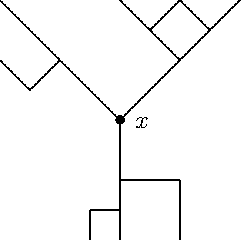
\includegraphics{pt}
\caption{$x$ é um ponto triplo}
\label{fig:pt}
\eef


a. Suponha que G seja um grafo conexo e que $x_1,x_2,\ldots,x_n$ sejam
pontos triplos distintos para G. Mostre que para algum i dois dos três
ramos em $x_i$, digamos $E_2(x_i)$ e $E_3(x_i)$ não contêm nenhum dos
outros pontos triplos ($\{x_1,\ldots,x_n\}\backslash\{x_i\}$).[Sugestão:
indução em n]

b. Considere o grafo $\mbox{G}'$ obtido de G e $x_1,\ldots,x_n$ do item anterior
remo\-ven\-do-se todos os sítios de $E_3(x_i)$ e todos os elos tocando estes
sítios. Mostre que $\{x_1,\ldots,x_n\}\backslash\{x_i\}$ são pontos triplos
para $\mbox{G}'$.

c. Suponha que G seja um grafo conexo e que $x_1,\ldots,x_n$ sejam pontos triplos
distintos de G. Entre os 3n ramos,
$$E_1(x_1),E_2(x_1),E_3(x_1),E_1(x_2),\ldots,E_3(x_n),$$
mostre que se pode achar pelo menos n+2 ramos {\em disjuntos}.

\vs

\noindent {\bf Prova da Proposição~\ref{prop:uni2}}

Suponha que $\p(\eta\geq3)>0$. Vamos procurar uma contradição.

Seja o evento
\beqnn
\fn\=\{\mbox{pelo menos três aglomerados infinitos abertos distintos}\\
&&\mbox{atingem $\qnm$}\}.
\eeqnn

Note que $\fn\uparrow\{\eta\geq3\}$ quando $n\uparrow\infty$, logo
existe $n_0$ tal que $\p(\fnu)>0$. Dados $\y$ três pontos distintos
no interior das faces de $\partial\qnu$, seja o evento
\beqnn
\fnu(\y)\=\{\y\,\,\mbox{pertencem a aglomerados infinitos distintos}\\
&&\mbox{usando apenas elos exteriores a $\qnu$}
\footnotemark\}.
\eeqnn
\footnotetext{exclui elos com pelo menos uma extremidade em $\qnm$}
Como $\fnu\subset\bigcup_{\y}\fnu(\y)$, temos que
\beq
\p(\fnu(\y))>0
\eeq
para algum $\y$. Dados estes $\y$, seja $x=x(\y)$ um ponto do interior
de $\qnu$ com a propriedade de que há três caminhos de elos disjuntos
no interior $\qnu$\footnote[2]{$\qnm$ mais os elos com uma extremidade
em $\qnm$} ligando $x$ a $\y$ respectivamente. Defina agora o evento
\beqnn
\fln(\y)\=\{\mbox{os três caminhos mencionados acima estão abertos,}\\
&&\mbox{todos os demais elos do interior de $\qn$ estão fechados}\}.
\eeqnn

\bef
%\input pte
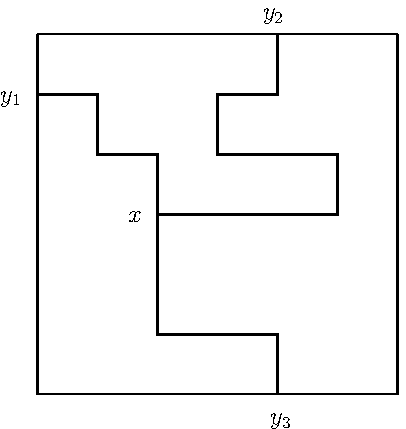
\includegraphics{pte}
\caption{O evento $\fln(\y)$.}
\eef

Logo 
\beqnn
&&\p(\fnu(\y)\cap\fln(\y))\\ \=\p(\fnu(\y))\p(\fln(\y))>0,
\eeqnn 
onde a
igualdade segue da independência dos eventos (o primeiro depende 
apenas de elos exteriores a $\qnu$; o segundo, apenas de elos interiores).

Vamos dizer agora que um ponto triplo (segundo a definição no exercício acima)
é um {\em ponto triplo especial} se seus ramos são infinitos.
Note que
$$
\{\mbox{$x(\y)$ é um ponto triplo especial}\}\supset\fnu(\y)\cap\fln(\y).
$$
De toda discussão acima, concluimos que, se $\p(\eta\geq3)>0$,
então
\beq
\p(\mbox{$x$ é um ponto triplo especial})>0.
\eeq
A probabilidade acima não depende de $x$, pela invariância por translação
de $\p$. Vamos denotá-la por $\rho$.
Segue-se que
\beq
\ep(\mbox{\#\{pontos triplos especiais em $\qnm$}\})=(2n-1)^d\rho,
\eeq
logo
\beq
\label{eq:con}
\p[\mbox{\#(pontos triplos especiais em $\qnm$})\geq(2n-1)^d\rho)]>0
\eeq
para todo $n$ (pois, para toda variável aleatória integrável X, 
$$P(X\geq E(X))>0).$$

Por outro lado, é uma conseqüência do exercício acima que o número de pontos
triplos especiais em $\qnm$ é inferior a $2d(2n-1)^{d-1}$ para toda
configuração de $\Om$ e todo $n$, o que contradiz 
(\ref{eq:con}) para $n$ suficientemente grande. 
Da contradição segue o resultado.

Vamos agora argumentar a afirmação no começo do parágrafo anterior.
Cada ramo de cada ponto triplo especial (pte) toca um (ou mais) sítios
em alguma face de $\partial\qn$ ($2d(2n-1)^{d-1}$ é o total de  
sítios em $\partial\qn$).

Considere os componentes conexos dos pte's usando apenas elos no interior
de $\qn$. Digamos que cada componente contenha $n_1,n_2,\ldots$ pte's
cada (isto é, o $i$-ésimo componente contem $n_i$ pte's). Logo
\beq
n_1+n_2+\ldots
\eeq
dá o total de pte's em $\qnm$.
Usando a linguagem do exercício acima, cada componente contem $n_i$ pontos
triplos. Daquele resultado sabemos que podemos achar pelo menos $n_i+2$
ramos distintos dentre as $3n_i$ possibilidades. Portanto, podemos achar
\beq
(n_1+2)+(n_2+2)+\ldots
\eeq 
ramos distintos de todos os pontos triplos. Como cada um toca pelo menos
um ponto das faces de $\qn$, será necessário que
\beq
n_1+n_2+\ldots\leq(n_1+2)+(n_2+2)+\ldots\leq2d(2n-1)^{d-1},
\eeq
como queríamos mostrar. $\bo$

\vspace{.5cm}

A seguir, apresentamos alguns corolários do Teorema~\ref{teo:uni}.
Lembramos que $\tau_p(x,y)$ é a função de conectividade dos sítios
$x$ e $y$, isto é,
$$\tau_p(x,y)=\p(x\leftrightarrow y).$$

\vs

\bco
\beq
\tau_p(x,y)\geq[\tep]^2
\eeq
\eco

\vs

O resultado acima tem como conseqüência que, na fase supercrítica,
a função de conectividade entre
dois pontos não decai quando a distância entre eles cresce.

\vs

\noindent {\bf Prova}

\beqnn
\tau_p(x,y)\ge\p(\mbox{$x$ e $y$ estão no mesmo aglomerado infinito})\\
\=\p(|C_x|=|C_y|=\infty)\geq\p(|C_x|=\infty)\p(|C_y|=\infty)=\tep^2,
\eeqnn
onde a primeira igualdade deve-se ao Teorema~\ref{teo:uni} e a última
desigualdade é FKG. $\bo$
\bco
$\tep$ é contínua à esquerda em $(p_c,1]$.
\eco

\noindent {\bf Prova}

Vamos construir modelos de percolação para todo $p\in[0,1]$ acoplados
usando uma família de variáveis i.i.d. Uniformes em $[0,1]$ 
$\{Z_e, e\in\ed\}$ declarando um elo $e$ $p$-aberto se $Z_e<p$
(como na prova da monotonicidade de $\tep$). Seja $C_p$ o aglomerado 
da origem com elos $p$-abertos.

Se $\pi\leq p$ então $\cpi\subset\cp$ e
\beqnn
\lim_{\pi\ua p}\tepi\=\lim_{\pi\ua p}\pp(|\cpi|=\infty)\\
\=\pp(\cup_{\pi<p}\{|\cpi|=\infty\}).
\eeqnn

Queremos mostrar que a última probabilidade acima vale $\tep$.
Consideremos então
\beq
\tep-\pp(\cup_{\pi<p}\{|\cpi|=\infty\})=\pp(|\cp|=\infty,|\cpi|<\infty\,
\forall\,\pi<p)
\eeq
para $p>p_c$. 
Para concluirmos que a última expressão é nula, basta argumentarmos que 
se $|\cp|=\infty$ e o aglomerado infinito $p$-aberto for único, então
$|\cpi|=\infty$ para algum $\pi<p$. 

De fato, nestas condições, tome $\a$ satisfazendo $p_c<\a<p$. Então,
quase certamente existe um aglomerado infinito $\a$-aberto, $\ia$, que
precisa satisfazer $\ia\sub\cp$ (pois do contrário haveria dois aglomerados
infinitos de elos $p$-abertos!). 

Logo, existe um caminho finito de elos $p$-abertos $\ga$ ligando a origem a
$\ia$. Como $\ga$ é finito e cada elo $e$ nele tem $Z_e<p$, então
$$\mu=\max\{Z_e,\,e\in\ga\}<p.$$ Se $\pi$ for tal que
$\pi\geq\a$ e $\mu<\pi<p$, então $\ia$ e $\ga$ são $\pi$-abertos.
Portanto $|\cpi|=\infty$.$\bo$

\vspace{.5cm}

O resultado acima, junto com o seguinte (que não é corolário da unicidade do
aglomerado infinito) nos diz que $\tep$ é contínua em $(\pce,1]$.

\bpro
\label{pro:cond}
$\tep$ é contínua à direita.
\epro

\vs

\noindent {\bf Prova}

Seja $A_n$ o evento de que a origem está ligada à fronteira de $\sn$ por um
caminho aberto. $(A_n)_{n\geq1}$ é uma seqüência decrescente e
$$\p(A_n)\downarrow\tep$$quando $n\uparrow\infty$. $\p(A_n)$ é contínua em $p$
(pois é um polinômio) e,
usando o modelo padrão do Capítulo 1, é fácil ver também que é crescente nesta
variável. Logo, $\tep$ é o limite decrescente de funções contínuas crescentes.
Um resultado de análise sobre funções semi-contínuas inferiores (ou um
argumento direto) nos dá o resultado. $\bo$

\bob
Como conseqüência dos dois últimos resultados, temos que $\tep$ será contínua
em $[0,1]$ se e somente se $\tepc=0$.
\eob

\vs

Para o próximo corolário, vamos dizer que ocorre um {\em cruzamento da esquerda para
a direita} no cubo $Q_n$ se houver um caminho de elos abertos contidos em $Q_n$
ligando a face esquerda de $Q_n$ a sua face direita. Denotemos por $\den$ o
evento de que tal cruzamento ocorre. $\den$ poderia ser visto como uma versão
a volume finito do evento de que há percolação. É uma decorrência do decaimento
exponencial do raio de $C$ na fase subcrítica que $\p(\den)\to0$ quando $n\to\infty$
neste caso (verifique). O caso supercrítico será tratado no próximo resultado.

\vs

\bco 
\label{cor:lrc}
Se $\tep>0$, então 
\beq
\p(\den)\to1
\eeq
quando $n\to\infty$.
\eco

\vs

Veremos no próximo capítulo que em $p=\pce$ um evento similar a $\den$
tem probabilidade que não converge
nem para 0 nem para 1 quando $n\to\infty$.

\vs

\noindent {\bf Prova}

Seja $I_m$ o evento de que algum sítio de $Q_m$ está num aglomerado infinito.
Dado $\eps>0$, escolha $m$ grande o suficiente para que 
\beq
\label{eq:lr1}
\p(I_m)>1-\eps
\eeq
(isto é possível pela discussão nos primeiros parágrafos do capítulo).

Temos que, para $n\geq m$
\beq
I_m\subset\cup_{i=1}^{2d}\left\{Q_m\lr F_i\,\mbox{em}\, Q_n\right\},
\eeq
onde $F_1,\ldots,F_{2d}$ são as faces de $Q_n$.

Logo
\beqn
\nonumber
1-\p(I_m)\ge1-\p\left(\cup_{i=1}^{2d}\left\{Q_m\lr F_i\,\mbox{em}\,
    Q_n\right\}\right)\\
\nonumber
\=\p\left(\cap_{i=1}^{2d}\left\{Q_m\lr F_i\,\mbox{em}\,
    Q_n\right\}^c\right)\\
\label{eq:lr2}
\ge\left[1-\p\left(Q_m\lr F\,\mbox{em}\,
    Q_n\right)\right]^{2d},
\eeqn
onde $F\in\{F_1,\ldots,F_{2d}\}$ e a última desigualdade segue de 
FKG pelo fato de que os eventos
na intersecção são decrescentes e também do fato que estes eventos
têm a mesma probabilidade (vide prova do Lema~\ref{le:leb1} na 
página~\pageref{le:leb1}).

De~(\ref{eq:lr1}) e~(\ref{eq:lr2}), temos que
\beq
\label{eq:lr3}
\p\left(Q_m\lr F\,\mbox{em}\,Q_n\right)\geq 1-\eps^{1/{2d}}
\eeq

Sejam $F_e$ e $F_d$ as faces esquerda e direita de $Q_n$ respectivamente.
Por FKG e~(\ref{eq:lr3}),
\beq
\p\left(\{Q_m\lr F_e\,\mbox{em}\,Q_n\}\cap\{Q_m\lr
  F_d\,\mbox{em}\,Q_n\}\right) \geq (1-\eps^{1/{2d}})^2
\eeq

Seja agora $\amn$ o evento de que há 2 sítios em $\del Q_m$ em 2 aglomerados
abertos disjuntos, ambos tocando $\del Q_n$. Temos que $\amn\supset\amnu$ e
$\amn\downarrow A_m$ quando $n\uparrow\infty$, onde $A_m$ é o evento de que
há 2 aglomerados abertos infinitos disjuntos tocando $Q_m$.

\bef
%\input amn
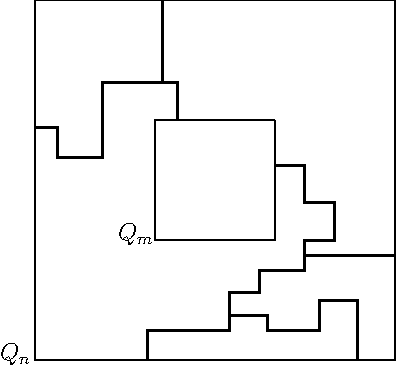
\includegraphics{amn}
\caption{O evento $\amn$}
\eef

Em conclusão
\beq
\p(\amn)\to\p(A_m)=0
\eeq
quando $n\to\infty$ e portanto, de
\beq
\p(\den)\geq (1-\eps^{1/{2d}})^2-\p(\amn),
\eeq
que decorre de
\beq
\{Q_m\lr F_e\,\mbox{em}\,Q_n\}\cap\{Q_m\lr
  F_d\,\mbox{em}\,Q_n\}\subset\den\cup\amn,
\eeq
temos
\beq
\liminf_{n\to\infty}\p(\den)\geq (1-\eps^{1/{2d}})^2
\eeq
e o resultado segue de $\eps$ ser arbitrário. $\bo$


















\chapter{O Modelo em 2 Dimensões: Dualidade}
\pagestyle{myheadings}
\markboth{CAPÍTULO 5.\quad DUAS DIMENSÕES}{DUALIDADE}
\setcounter{equation}{0}
\label{chp:bid}
Neste capítulo e no próximo, vamos tratar do que ocorre em $p=\pce$.
Em 2 dimensões, objeto deste capítulo, a auto-dualidade da rede $\zt$ 
permite mostrar que $\pce=1/2$ e $\theta(\pce)=0$, o que estabelece a
continuidade de $\tep$ em todo o intervalo $[0,1]$. 
Além da dualidade da rede bidimensional, outros 
ingredientes da prova são o decaimento exponencial da distribuição 
do raio de $C$ em $p<\pce$ (Teorema~\ref{teo:teo1}) e a unicidade do 
aglomerado infinito em $\tep>0$ (Teorema~\ref{teo:uni}).

Consideremos de novo, como na demonstração da Proposição~\ref{prop:trans2} 
(na página~\pageref{trans2}), a rede bidimensional dual de $\zt$, 
$$\zs=\zt+\{1/2,1/2\}.$$
$\zs$ é isomorfa a $\zt$ (por isto dizemos que $\zt$ é auto-dual).
Este fato é crucial para o que se segue. Outro fato crucial, que
já usamos na demonstração da Proposição~\ref{prop:trans2}, é a 
seguinte propriedade geométrica de $\zt$.

\vs

\bpro
\label{pro:geo}
Seja $G$ um subgrafo conexo finito de $\zt$. Existe um único circuito
$\Gamma$ de $\zs$ contendo $G$ com a propriedade de que todo elo de
$\Gamma$ cruza um elo de $\Delta G$, a fronteira de $G$ (isto é, os
elos de $\zt\backslash G$ que incidem em pelo menos um sítio de $G$).
\epro

\vs


\bte
\label{teo:2d}
Em duas dimensões,
\beqnn
\pce=1/2\quad\mbox{e}\quad\theta(\pce)=0.
\eeqnn
\ete

\vs

O Teorema~\ref{teo:2d} será provado por meio dos dois seguintes lemas.

\vs

\ble
\label{le:leb1}
Em duas dimensões,
\beqnn
\theta(1/2)=0.
\eeqnn
\ele

\vs

\bob
Este resultado tem a conseqüência imediata que em dimensão 2$$\pce\geq1/2.$$
\eob

\vs

\ble
\label{le:leb2}
Em duas dimensões,
\beqnn
\pce\leq1/2.
\eeqnn
\ele

\vs

A heurística para a validade do primeiro lema é que, se $\theta(1/2)>0$, 
então teremos um aglomerado infinito aberto em $\zt$ e 
um aglomerado infinito fechado em $\zs$. Os dois aglomerados não podem
se tocar (lembre que os elos de $\zs$ têm o mesmo status que os respectivos
elos secantes de $\zt$ --- vide a demonstração da Proposição~\ref{prop:trans2}
na página~\pageref{trans2}) e $\zt$ é pequeno demais para isto.

Para o segundo lema, a heurística é que em $p<\pce$, há apenas aglomerados
abertos finitos (ilhas) em $\zt$ num {\em mar} de elos fechados do dual.
Presumivelmente estes formam um aglomerado infinito. Logo, $1-p\geq\pce$
sempre que $p<\pce$, o que implica no resultado do lema.


\vs

\noindent{\bf Prova do Lema~\ref{le:leb1}}

O argumento, não publicado, é de Y. Zhang.
Usaremos o {\em truque da raiz quadrada} de Cox \& Durrett (já usado no
capítulo anterior na demonstração do Corolário~\ref{cor:lrc}): Se 
$$A_1,\ldots,A_m$$ forem eventos crescentes de mesma probabilidade então
$$1-\p(\cup_{i=1}^mA_i)=\p(\cap_{i=1}^mA_i^c)\geq[1-\p(A_1)]^m,$$
onde a desigualdade é FKG.
Logo
$$\p(A_1)\geq1-[1-\p(\cup_{i=1}^mA_i)]^{1/m}.$$

Suponha que 
\beq
\label{eq:abs}
\th>0.
\eeq

Seja $\aen$ o evento de que algum sítio do lado esquerdo de $\tn=[0,n]^2$
esteja num aglomerado aberto infinito de $\zt$ {\em sem} usar outros sítios de
$\tn$. Defina $\adn$, $\acn$ e $\abn$ similarmente substituindo lado esquerdo
por lado direito, lado de cima e lado de baixo, respectivamente.

Como conseqüência de~(\ref{eq:abs})
$$\ph(\mbox{existir um aglomerado aberto infinito})=1$$
de onde concluimos que
$$\ph(\aen\cup\adn\cup\acn\cup\abn)\to1$$quando $n\to\infty.$

Pelo truque da raiz quadrada,
\beq
\ph(\aun)\to1
\eeq
quando $n\to\infty$ para $u=e,d,c,b$.

Escolhamos $N$ tal que 
\beq
\label{eq:abs1}
\ph(\Anu)>7/8\quad\mbox{e}\quad\ph(\Anou)>7/8
\eeq
para $u=e,d,c,b$.

Na rede dual, sejam
$\asen$ o evento de que algum sítio do lado esquerdo de $\tsn=[0,n-1]+(1/2,1/2)$
esteja num aglomerado {\em fechado} infinito de $\zs$ {\em sem} usar outros sítios de
$\tsn$ e $\asdn$, $\ascn$ e $\asbn$ similarmente definidos substituindo lado esquerdo
por lado direito, lado de cima e lado de baixo, respectivamente.

Temos 
\beq
\label{eq:abs2}
\ph(\asnu)=\ph(\Anou)>7/8.
\eeq

Considere $$A=\ane\cap\adn\cap\asnc\cap\asnb.$$ 
Note que, em $A$, se houver apenas um
aglomerado infinito aberto em $\zt$ e apenas um aglomerado infinito fechado em $\zs$
então os caminhos abertos infinitos à esquerda e à direita de $\tne$ devem se ligar por elos
abertos por dentro
de $\tsne$ pois por fora os caminhos infinitos fechados acima e abaixo de $\tsne$ bloqueiam
a passagem. Similarmente, os caminhos infinitos fechados acima e abaixo de $\tsne$ devem se ligar
por elos fechados por dentro de $\tne$. Mas neste caso, as ligações por dentro de $\tne$ e 
$\tsne$
devem se cruzar, o que é impossível. Logo, em $A$ há dois aglomerados infinitos abertos 
disjuntos em $\zt$ ou dois aglomerados infinitos fechados disjuntos em $\zs$
(veja a Figura~\ref{fig:bid1}). Concluimos do Teorema~\ref{teo:uni} que 
\beq
\label{eq:zh}
\p(A)=0.
\eeq

\bef
%\input zh
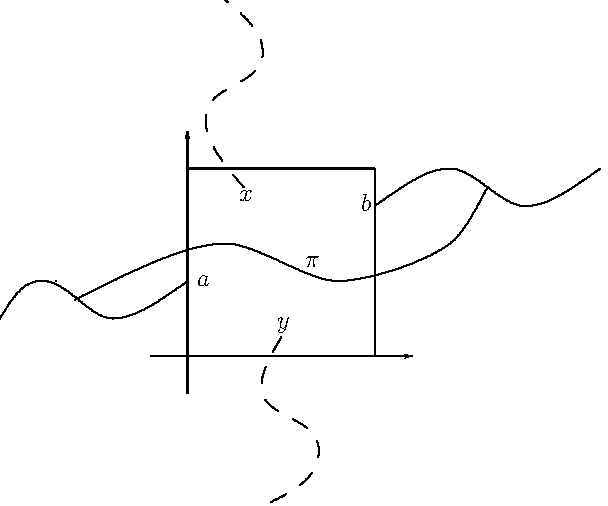
\includegraphics{zh}
\caption{Os sítios $a$ e $b$ estão em aglomerados abertos infinitos de
  $\zt\backslash T_N$ e os sítios $x$ e $y$ estão em aglomerados fechados infinitos de
  $\zs\backslash T_N^\ast$. Se houver um único aglomerado aberto infinito,
  então existe um caminho aberto $\pi$ ligando $a$ a $b$, e então os
  aglomerados infinitos fechados em $x$ e $y$ são disjuntos.}
\label{fig:bid1}
\eef

Por outro lado
\beqnn
\ph(A^c)\le\ph[(\ane)^c]+\ph[(\adn)^c]+\ph[(\asnc)^c]+\ph[(\asnb)^c]\\
\le1/2
\eeqnn
por~(\ref{eq:abs1}) e~(\ref{eq:abs2}).Logo, $\p(A)\geq1/2$, em contradição com~(\ref{eq:zh}), o que prova o lema. $\bo$





\vs





\noindent{\bf Prova do Lema~\ref{le:leb2}}

Vamos mostrar que, se $p<\pce$, então existe um aglomerado fechado infinito no
dual com probabilidade positiva, o que implica que $1-p\geq\pce$, o que por
sua vez produz o resultado do lema.

Se $p<\pce$, então do Corolário~\ref{cor:exp} temos que
\beq
\label{eq:deca}
\xip=\sum_{n=1}^\infty\p(|C|\geq n)<\infty.
\eeq
Seja $M$ um inteiro positivo e
\beqnn
\am&\!\!=&\!\!\{\mbox{Existe um caminho aberto $\pi$ em $\zt$ ligando 
algum sítio da forma}\\
&&\,\,\mbox{$(k,0)$ com $k<0$ a algum outro da forma  $(l,0)$ com
$l\geq M$ com a}\\
&&\,\,\mbox{propriedade de que todos os elos de $\pi$, a não
ser os extremos,}\\
&&\,\,\mbox{estão acima do eixo horizontal}\}
\eeqnn

\bef
%\input am
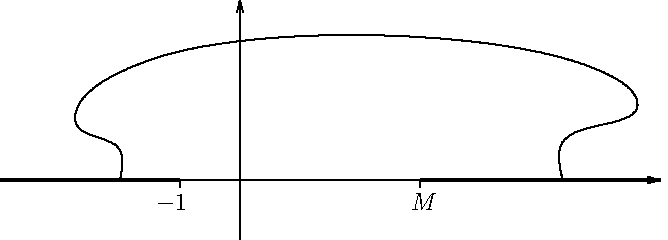
\includegraphics{am}
\caption{Um esboço do evento $\am$}
\eef

Então
\beqnn
\p(\am)\le\p\left(\bigcup_{l=M}^\infty\{(k,0)\lr(l,0)\,\,\mbox{para
    algum}\,\,k<0\}\right)\\
\le\sum_{l=M}^\infty\p((k,0)\lr(l,0)\,\,\mbox{para algum}\,\,k<0)\\
\=\sum_{l=M}^\infty\p((0,0)\lr(k-l,0)\,\,\mbox{para algum}\,\,k<0)\\
\=\sum_{l=M}^\infty\p((0,0)\lr(l+m,0)\,\,\mbox{para algum}\,\,m>0)\\
\le\sum_{l=M}^\infty\p(|C|\geq l).
\eeqnn
(\ref{eq:deca}) nos permite escolher $M$ tal que
\beq
\p(\am)\leq1/2.
\eeq

%Em $\am^c$ existe um aglomerado fechado infinito em $\zs$.

Seja agora $$L=\{(m+1/2,1/2):-1\leq m<M\}.$$ Denote por $C(L)$ o conjunto de sítios
do dual conectados a $L$ por caminhos fechados do dual.

Se $|C(L)|<\infty$, então existe um circuito aberto no dual de $\zs$, isto é
$\zt$, ao redor de $C(L)$ (pela Proposição~\ref{pro:geo}). Logo deve haver um
caminho aberto em $\zt$ ligando sítios do tipo $(k,0)$ com $k<0$ e $(l,0)$ com
$l\geq M$ inteiramente no semiplano superior. Então
\beq
\p(|C(L)|<\infty)\leq\p(\am)\leq1/2.
\eeq
Portanto $\p(|C(L)|=\infty)\geq1/2$. Mas então pelo menos um sítio de $L$ tem
que estar num aglomerado fechado infinito. De onde se conclui que
\beqnn
\p(\mbox{$0_\ast$ está num aglomerado fechado
infinito})\ge\frac{1}{M+1}\p(|C(L)|=\infty)\\
\ge\frac{1}{2(M+1)}
\eeqnn
e o lema está provado. $\bo$

\vs

A seguir apresentaremos uma outra prova do mesmo lema que tem um interessante
subproduto.

\vs


\noindent{\bf Outra prova do Lema~\ref{le:leb2}}

Considere os seguintes conjuntos de sítios
\beqnn
\Lambda_n\=\{x\in\zt:0\leq x_1\leq n+1,\,0\leq x_2\leq n\}\\
\Lambda_n^\ast\=\{x+(1/2,1/2),\,x\in\zt:0\leq x_1\leq n,\,-1\leq x_2\leq n\},
\eeqnn 
os subgrafos
\begin{eqnarray*}
S_n=\Lambda_n&\cup&\{\mbox{elos vizinhos mais próximos de $\Lambda_n$ exceto}\\
&&\quad\mbox{$(x,y)$ com $x_1=y_1=0$ ou $x_1=y_1=n+1$}\}\\
S_n^\ast=\Lambda_n^\ast&\cup&\{\mbox{elos vizinhos mais próximos de
$\Lambda_n^\ast$ exceto}\\
&&\quad\mbox{$(x,y)$ com $x_2=y_2=-1$ ou $x_2=y_2=n$}\}
\end{eqnarray*}
e os eventos
$A_n$ de que existe um caminho aberto em $S_n$ ligando seu lado esquerdo a seu lado
direito e $A_n^\ast$ de que existe um caminho fechado em $S_n^\ast$ ligando seu
lado de baixo a seu lado de cima.

\bef
%\input s5
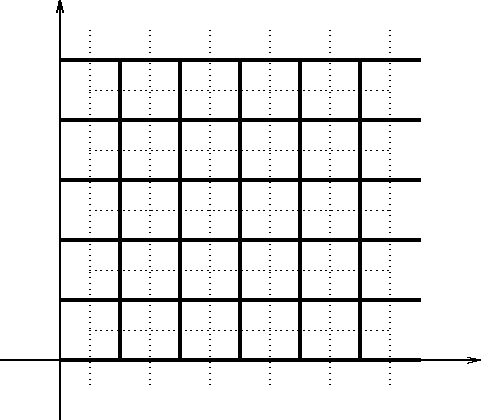
\includegraphics{s5}
\caption{$S_5$ e seu dual $S_5^\ast$}
\eef

Temos que
\beq
\label{eq:dis}
\an\cap\asn=\emptyset
\eeq
pois senão haverá um cruzamento entre caminho aberto em $\sn$ com caminho
fechado de $\ssn$, o que é impossível.

Por outro lado
\beq
\label{eq:exa}
\an\cup\asn=\Omega.
\eeq
De fato, suponha que $\an$ não ocorre. Seja $D$ o conjunto de sítios de $\sn$
alcançados da face esquerda junto com os elos ligando tais sítios.
Por uma variante da Proposição~\ref{pro:geo}, existe um caminho em
$\zs$ cruzando $\ssn$ de cima a baixo secante apenas a elos de $\sn$ contidos
na fronteira de $D$. Logo este caminho será fechado e $\asn$ ocorre (veja
Figura~\ref{fig:bid3}).

\bef
%\input du2
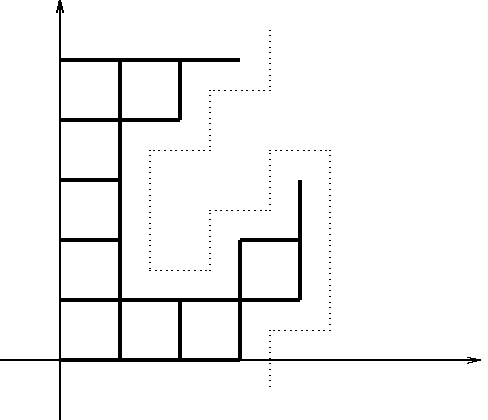
\includegraphics{du2}
\caption{Ilustração do fato de que se não há caminhos abertos atravessando 
  $\sn$ da esquerda para a
  direita, então há um caminho fechado cruzando $\ssn$ de cima para baixo.}
\label{fig:bid3}
\eef

De~(\ref{eq:dis}) e~(\ref{eq:exa})
\beq
\p(\an)+\p(\asn)=1.
\eeq
Mas $\p(\asn)=P_{1-p}(\an)$. Logo
\beq
\ph(\an)=1/2
\eeq
(para todo $n$).

Mas se $\pce>1/2$, então $\ph(\an)\to0$ quando $n\to\infty$
(por uma variante do argumento que diz que $\p(\den)\to0$
quando $n\to\infty$ se $p<\pce$ mencionado no capítulo anterior).

A contradição prova o lema. $\bo$

\vs

O subproduto interessante desta prova a que se aludiu acima é o fato
de que $\ph(A_n)=1/2$ independentemente de $n$.
Pode-se argumentar (faça-o) como para $\den$ que 
$$\p(\an)\to 0\quad\mbox{ou}\quad 1$$
quando $n\to\infty$ conforme $p<\pce$ ou $p>\pce$ respectivamente.







\chapter{Continuidade no Ponto Crítico: Renormalização}
\pagestyle{myheadings}
\markboth{CAPÍTULO 6.\quad NO PONTO CRÍTICO}{RENORMALIZAÇÃO}
\setcounter{equation}{0}
\label{chp:ren}
Neste último capítulo trataremos de forma pincelada de um método de ataque
ao problema de se provar a continuidade de $\tep$ em $\pce$ em mais dimensões
do que duas. Neste caso, não temos nem a auto-dualidade da rede
hipercúbica nem conhecemos (ou esperamos algum dia conhecer) o valor exato
de $\pce$. Ambos conhecimentos foram úteis em $d=2$ (Capítulo~\ref{chp:bid}).

A idéia será relacionar a ocorrência de percolação a um evento {\em em volume
finito}, cuja probabilidade, sendo contínua (pois as probabilidades de todos
tais eventos são polinômios em $p$), nos permitirá concluir que, se há 
percolação para $p$, então há também para $p-\eps$ com $\eps>0$ 
suficientemente pequeno.

O método é chamado de {\em renormalização}. A versão a ser esboçada, que chamaremos
renormalização {\em estática}, não foi ainda realizada com rigor em modelos
de percolação (uma prova para a Proposi\c cão~\ref{pro:ren2} abaixo
ainda não
foi feita), mas técnicas de renormalização {\em dinâmica} muito similares
foram aplicadas
com sucesso para percolação em semi-espaços de $\bbz^d$, $d\geq3$ 
\cite{kn:BGN}. O problema da continuidade no ponto crítico
em $\zd$ inteiro permanece aberto para valores intermediários de $d$ entre
$2$ e $d_0$, este último o menor valor para o qual Hara e Slade \cite{kn:HS} podem
aplicar sua {\em expansão em laços} e obter a continuidade a partir daí, entre outros 
resultados ($d_0$ estava em 19 segundo as últimas notícias,
mas não se espera que possa vir abaixo de 7).

Para $0\leq K\leq L$, considere a partição de $\zd$ em cubos concêntricos 
de lado $2K$ e $2L$ como na figura abaixo e seja $\akl$ o evento em que
existe um caminho aberto dentro dos dois cubos grandes conectando a superfície
dos dois cubos menores (vide Figura~\ref{fig:fren1}).

\bef
%\input fren1
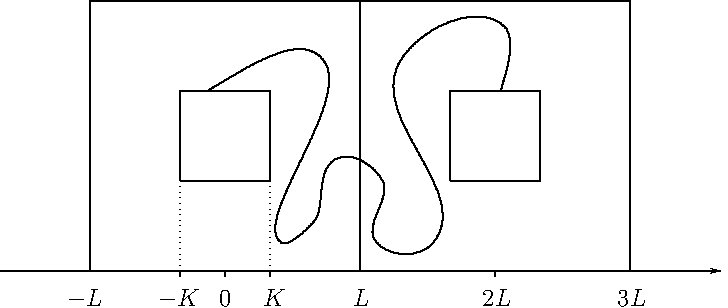
\includegraphics{fren1}
\caption{O evento $\akl$}
\label{fig:fren1}
\eef

Para garantir interconexão, precisamos intersectar $\akl$ com outro e\-ven\-to
$$\bkl=\bklu\cap\bkld,$$
em que $\bkli$, $i=1,2$, é o evento de que todos os sítios do cubo menor $i$, que
estiverem ligados por caminhos abertos à fronteira do cubo grande respectivo,
estarão conectados entre si por caminhos abertos dentro do cubo grande.

Seja $\aklt=\akl\cap\bkl$.

\vs

\bpro
\label{pro:ren1}
Seja $\rkl=\p(\aklt).$ Existe $\ls\in(0,1)$ tal que se (para algum $0\leq
K\leq L$ e $0<p<1$) $\rklp>\ls$, então $\tep>0$.
\epro
Um argumento para a validade deste resultado será esboçado adiante.

\vs

\bpro[Conjectura]
\label{pro:ren2}
Se, para algum $p'\in(0,1)$, $\tepl>0$, então
\beq
\label{eq:ren1}
\sup_K\liminf_{L\to\infty}P_{p'}(\akl)=1.
\eeq
\epro

\vs

\bte
\label{teo:ren}
Se a Proposição~\ref{pro:ren2} conjecturada for verdadeira, então $$\tepc=0.$$
\ete

\noindent{\bf Prova do teorema.}

Primeiro mostraremos que a Proposição~\ref{pro:ren2} conjecturada implica que
se $\tepl>0$, então 
\beq
\label{eq:ren2}
\sup_K\liminf_{L\to\infty}\rklpl=1
\eeq
(portanto $\rklpl>\ls$ para algum $K$ e $L$).

De fato, para cada $K$ fixo, $$\lim_{L\to\infty}\ppl(\bkli)=1$$
para $i=1,2$, pois de outra forma haveria probabilidade positiva de que 2
sítios do cubo menor estivessem em aglomerados infinitos disjuntos.
Logo $$\lim_{L\to\infty}\ppl(\bkl)=1$$ do que se conclui que
$$\lim_{L\to\infty}\ppl(\aklt)=\lim_{L\to\infty}\ppl(\akl)=1.$$

Agora suponha que, para algum $p'$, $\tepl>0$. Pelo argumento acima podemos
escolher $K_0$ e $L_0$ tais que $\rko>\ls$. Mas $\rkop$ é um polinômio em
$p$. Logo $$\rkoe>\ls$$ para algum $\eps$ positivo. Pela Proposição~\ref{pro:ren1}
$$\teple>0.$$

Temos portanto que $\tepl>0$ implica que $\teple>0$ para algum $\eps>0$.
Logo $\tepc$ não pode ser positivo, pois isto implicaria em $\tep$ positivo
para algum $p<\pce$, o que contradiz a definição de $\pce$. $\bo$

\vs

\noindent{\bf (Esboço de) Prova da Proposição~\ref{pro:ren1} (em $d=3$).}

Considere uma rede {\em renormalizada} isomórfica a $\zt$ na qual cada sítio
corresponde a um cubo $2L\times2L\times2L$ em $\bbz^3$, como na
Figura~\ref{fig:fren2}. Declare um elo
{\em renormalizado} aberto se $\aklt(e)$ ocorrer. 

\bef
%\input fren2
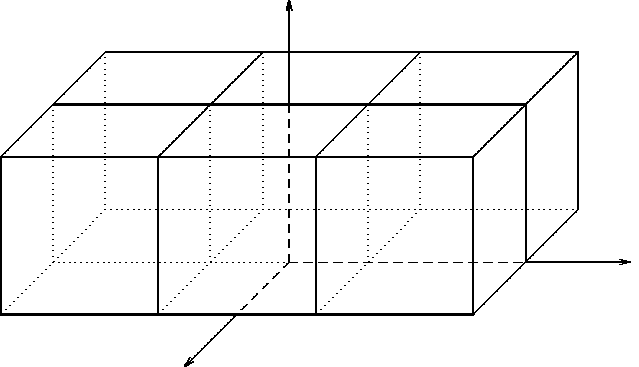
\includegraphics{fren2}
\caption{Parte da rede $\zt$ renormalizada.}
\label{fig:fren2}
\eef

Teremos então um modelo de percolação {\em dependente} na rede renormalizada
com uma medida de probabilidade $\ppt$ tal que 
$$\ppt(\mbox{$e$ está aberto})=\rkl.$$

Precisamos mostrar que existe $\ls\in(0,1)$ tal que se $\rkl$ for maior do 
que $\ls$, então
percolação dependente ocorre na rede renormalizada. Se isto ocorrer,
obviamente percolação independente ocorrerá na rede original.

A prova de que percolação dependente ocorre em $\zt$ renormalizada pode ser feita 
pelo mesmo argumento de Peierls na prova da Proposição~\ref{prop:trans2}
(a partir dos circuitos nos elos duais de $\zt$)
com a única pequena modificação de que a medida nos elos não é mais
independente, mas apenas {\em localmente} dependente. Deixamos os detalhes 
para o leitor. $\bo$


\appendix

\chapter{Prova a um lema do Capítulo 3}
\pagestyle{myheadings}
\markboth{APÊNDICE}{LEMA DO CAPÍTULO 3}
\setcounter{equation}{0}
\label{app}














Neste apêndice, provaremos o Lema~\ref{le:app} a partir de~(\ref{eq:eq3}).
Isto é, queremos mostrar que
para $p<\pce$, existe uma constante $\delp$ tal que
\beq
\label{eq:a1}
\gpn\leq\delp n^{-1/2}
\eeq

a partir de
\beq 
\label{eq:a2} 
\gan\leq\gbn\exp\left[(\b-\a)-(\b-\a)\frac{n}{\sum_{i=0}^ng_\beta(i)}\right], 
\eeq 
para $0\leq\a\leq\b<\pce$.
Além de~(\ref{eq:a2}), os únicos fatos requeridos pelo argumento são
\beqn
\label{eq:c1}
\mbox{$0<\gpn<1$ para todo $n$ e $p\in[0,\pce)$,}\\
\label{eq:c2}
\mbox{$\gpn$ é não-decrescente em $p$ para todo $p\in[0,\pce)$,}\\
\label{eq:c3}
\mbox{$\gpn$ é não-crescente em $n$ para todo $p\in[0,\pce)$ e}\\
\label{eq:c4}
\gpn\to0\quad\mbox{quando $n\to\infty$ e $p\in[0,\pce)$.}
\eeqn

\vs

\noindent{\bf Prova de~(\ref{eq:a1})}

Reproduzimos o argumento em \cite{kn:G}. Vamos primeiro escolher uma 
subseqüência $n_1,n_2,\ldots$ ao longo da qual $\gpn$ converge a $0$
bastante rápido. A seguir, fechamos as lacunas.

Fixemos $\b<\pce$ e um inteiro positivo $n$. Sejam $\a$ tal que $0<\a<\b$ e
$n'\geq n$. Adiante escolheremos $\a$ e $n'$ explicitamente em termos de $\b$.

De~(\ref{eq:a2}),
\beqn
\nonumber
\gal\le\gbl\exp\left(1-\frac{n'(\b-\a)}{\sum_{i=0}^{n'}\gbi}\right)\\
\label{eq:exp}
\le\gbn\exp\left(1-\frac{n'(\b-\a)}{\sum_{i=0}^{n'}\gbi}\right)
\eeqn
pois $n\leq n'$. Queremos escrever o expoente em termos de $\gbn$ e para
isto escolheremos $n'$ apropriadamente. Vamos quebrar a soma em duas partes,
para $i<n$ e $i\geq n$. Usando~(\ref{eq:c3}), temos
\beqnn
\frac{1}{n'}\sum_{i=0}^{n'}\gbi\le\frac{1}{n'}\{n\gbo+n'\gbn\}\\
\le3\gbn
\eeqnn
se $n'\geq n\lfloor\gbn^{-1}\rfloor$. Vamos definir agora
\beq
\label{eq:ga}
n'=n\gabn
\eeq
onde $\gabn=\lfloor\gbn^{-1}\rfloor$ e
deduzir de~(\ref{eq:exp}) que
\beq
\label{eq:gal}
\gal\leq\gbn\exp\left(1-\frac{\b-\a}{3\gbn}\right).
\eeq
Escolhemos a seguir $\a$ fazendo
\beq
\label{eq:al}
\b-\a=3\gbn\{1-\log\gbn\}.
\eeq
De~(\ref{eq:c4}) temos $0<\a<\b$ se $n$ for escolhido bastante grande.

De~(\ref{eq:gal}) temos
\beq
\label{eq:gal1}
\gal\leq\gbn^2.
\eeq
Usaremos esta conclusão recursivamente a seguir. Mostramos até agora
que, para $\b<\pce$ existe $\nob$ tal que~(\ref{eq:gal1}) vale sempre que
$n\geq\nob$ e $\a$ e $n'$ forem dados por~(\ref{eq:al}) e~(\ref{eq:ga})
respectivamente.

Fixemos agora $p<\pce$ e escolhamos $\pi$ tal que $p<\pi<\pce$. Construimos 
agora seqüências $(\pei,\,i\geq0)$ de probabilidades e $(\eni,\,i\geq0)$ de
inteiros. Façamos $p_0=\pi$ e deixemos $n_0$ para mais tarde. Tendo encontrado
$p_0,p_1,\ldots,\pei$ e $n_0,n_1,\ldots,\eni$, definimos
\beq
\label{eq:ind}
\enu=\eni\gai\quad\mbox{e}\quad \pei-\peu=3\gi(1-\log\gi)
\eeq
onde $\gi=\gpin$ e $\gai=\lfloor\gi^{-1}\rfloor$. Note que $\eni\leq\enu$ 
e $\pei>\peu$.

A recursão em~(\ref{eq:ind}) é válida enquanto $\peu>0$ e este será o caso se
$n_0$ for escolhido suficientemente grande. Para ver isto, argumentamos da seguinte 
forma. Da definição de $p_0,\ldots,\pei$ e $n_0,\ldots,\eni$ e da discussão que levou
a~(\ref{eq:gal1}) temos
\beq
\label{eq:gal2}
\gju\leq\gj^2
\eeq
para $j=0,1,\ldots,i-1.$ Se uma seqüência de números reais
$(\xj,\,j\geq0)$ satisfizer $0<x_0<1,\,x_{j+1}=\xj^2$ para $j\geq0$, então é fácil de 
ver que 
\beqnn
s(x_0)=\sum_{j=0}^\infty3\xj(1-\log\xj)<\infty
\eeqnn
e que $s(x_0)\to0$ quando $x_0\to0$. Podemos então tomar $x_0$ pequeno o suficiente para 
que
\beq
\label{eq:xo}
s(x_0)\leq\pi-p
\eeq
e depois tomar $n_0$ grande o suficiente para que $\go=\gpio<\xo$.
Agora $\hx=3x(1-\log x)$ é uma função crescente em $[0,\xo]$, o que junto 
com~(\ref{eq:ind}) e~(\ref{eq:gal2}) implica
\beqnn
\peu\=\pei-3\gi(1-\log\gi)\\
\=\pi-\sum_{j=0}^i3\gj(1-\log\gj)\\
\ge\pi-\sum_{j=0}^i3\xj(1-\log\xj)\\
\ge p
\eeqnn
por~(\ref{eq:xo}).

Desta forma, escolhendo $n_0$ convenientemente, teremos $\peu>0$ para
todo $i$ e também 
\beqnn
\ptil=\lim_{i\to\infty}\pei
\eeqnn
satisfazendo $\ptil\geq p$. Vamos supor que $n_0$ foi escolhido da forma adequada.
Temos então a recursão~(\ref{eq:ind}) válida e $\ptil\geq p$. De~(\ref{eq:ind})
e~(\ref{eq:gal2}) temos
\beqnn
\nk=n_0\ga_0\ga_1\ldots\ga_{k-1}
\eeqnn
para $k\geq1$ e
\beqn
\nonumber
g_{k-1}^2\=g_{k-1}g_{k-1}\\
\nonumber
\le g_{k-1}g_{k-2}^2\leq\cdots\\
\nonumber
\le g_{k-1}g_{k-2}\ldots g_1 g_0^2\\
\nonumber
\le (\ga_{k-1}\ga_{k-2}\ldots \ga_0)^{-1} g_0\\
\label{eq:gal3}
\=\d^2\nk^{-1},
\eeqn
onde $\d=n_0 g_0$.

O argumento está basicamente terminado. Seja $n>n_0$. Seja $k$ um inteiro tal que
$n_{k-1}\leq n<\nk$, o que é possível pois $g_k\to0$ quando $k\to\infty$ e logo
$n_{k-1}<\nk$ para todo $k$ bastante grande. Então
\beqnn
\gpn\le g_{p_{k-1}}(n_{k-1})\quad\mbox{pois $p\leq p_{k-1}$}\\
\=g_{k-1}\\
\le\d\nk^{-1/2}\quad\mbox{por~(\ref{eq:gal3})}\\
\le\d n^{-1/2}\quad\mbox{pois $n<\nk$}
\eeqnn
como queríamos. Isto vale para $n>n_0$. Ajustando a constante, temos a
desigualdade para todo $n$. $\bo$













%\bibliographystyle{apalike} 
\addcontentsline{toc}{chapter}{Referências Bibliográficas}

\pagestyle{myheadings}
\markboth{BIBLIOGRAFIA}{}

\begin{thebibliography}{99}

\bibitem{kn:BH} Broadbent, S.R. e Hammersley, J.M.,  Percolation processes I.
Crystals and mazes, {\em Proceedings of the Cambridge Philosofical Society}
{\bf 53} 629-641 (1957)
 
\bibitem{kn:H} Harris, T., A lower bound for the critical probability in a
  certain percolation process, {\em Proceedings of the Cambridge Philosofical Society}
{\bf 56}, 13-20 (1960)

\bibitem{kn:K1} Kesten, H., The critical probability of bond percolation on
  the square lattice equals $\frac{1}{2}$, {\em Communications in Mathematical
    Physics} {\bf 74}, 41-59 (1980)

\bibitem{kn:M} Menshikov, M.V., Coincidence of critical points in percolation
problems, {\em Soviet Mathematics Doklady} {\bf 33}, 856-859 (1986)

\bibitem{kn:AB} Aizenman, M. e Barsky, D., Sharpness of the phase transition
  in percolation models, {\em Communications in Mathematical
    Physics} {\bf 108}, 489-526 (1987)

\bibitem{kn:AKN} Aizenman, M., Kesten, H. e Newman, C.M., Uniqueness of the
  infinite cluster and continuity of connectivity functions for short- and
  long-range percolation, {\em Communications in Mathematical
    Physics} {\bf 111}, 505-532 (1987)

\bibitem{kn:BGN} Barsky, D., Grimmett, G. e Newman, C.M.,
Percolation in half-spaces: Equality of critical densities and continuity of
the percolation probability, {\em Probability Theory and Related Fields}
{\bf 90}, 111-148 (1991)

\bibitem{kn:G} Grimmett, G.R., {\em Percolation}, Springer (1989)

\bibitem{kn:B} Breiman, L., {\em Probability}, Addison-Wesley (1968)

\bibitem{kn:K2} Kesten, H., {\em Percolation Theory for Mathematicians}, 
                Birkhäuser (1982)

\bibitem{kn:K3} Kesten, H., Asymptotics in high dimensions for percolation, 
{\em Disorder in physical systems}, 219--240, Oxford University Press (1990) 

\bibitem{kn:FKG} Fortuin, C.M., Kasteleyn, P.W., e Ginibre, J., Correlation
  inequalities on some partially ordered sets, {\em Communications in Mathematical
    Physics} {\bf 22}, 89-103 (1971)

\bibitem{kn:vBK} van den Berg, J. e Kesten, H., Inequalities with applications
  to percolation and reliability, {\em Journal of Applied Probability} {\bf
    22}, 556-569 (1985)

\bibitem{kn:R} Russo, L., On the critical percolation probabilities,
{\em Zeitschrift für Wahrscheinlichkeitstheorie und Verwandte Gebiete} 
{\bf 56}, 229-237 (1981)

\bibitem{kn:NS} Newman, C.M. e Schulman, L.S., 
                Infinite clusters in percolation models,  
                {\em Journal of Statistical Physics} {\bf 26}, 613--628 (1981)

\bibitem{kn:BK} Burton, R.M. e Keane, M., Density and uniqueness in
  percolation, {\em Communications in Mathematical Physics} {\bf 121},
501-505 (1989)

\bibitem{kn:HS} Hara, T. e Slade, G., Mean-field critical behavior for
  percolation in high dimensions, {\em Communications in Mathematical
    Physics} {\bf 128}, 333-391 (1990)

\end{thebibliography}


\end{document}


